%!TEX root = Manuscrit.tex
\section{Apprentissage profond pour la vision artificielle}

\subsection{Historique de l'apprentissage profond}

La possibilité d'attribuer des capacités cognitives à un ordinateur a été originellement formalisé par Alan Turing en 1950~\cite{turing_computing_1950}. Turing propose un cadre formel permettant de répondre à la question \og{} une machine peut-elle penser \fg{} en définissant ce qui est désormais connu comme le test de Turing. Selon lui, un ordinateur intelligent serait défini par sa capacité à imiter un humain de manière à ce que d'autres individus soient incapables de discerner sa véritable nature. Toutefois, Turing ne répond pas à la question du \og comment \fg{} et ne propose pas d'implémentation permettant d'atteindre cet objectif.

Néanmoins, en 1943, Warren McCulloch et Walter Pitts proposaient un système de neurones booléens~\cite{mcculloch_logical_1943} munis de deux état\,: actifs ou inactifs. Ils définissent un neurone formel comme étant un automate fini muni d'une fonction de transfert, permettant de transformer un ensemble d'entrée en une valeur de sortie. Certains neurones ne recevaient aucun signal d'un autre neurone, mais formaient eux-mêmes l'ensemble du signal d'entrées pour le reste du réseau. Les autres neurones calculaient alors des combinaisons logiques à partir des signaux qu'ils recevaient en entrée. Les travaux de McCulloch et Pitts montrent que de nombreux prédicats de logique temporelle sont calculables par de tels réseaux booléens. Cette étude théorique est étendue par Kleene qui étudie notamment des réseaux booléens dont le graphe présente des cycles, c'est-à-dire des réseaux \emph{récurrents}. Kleene montre notamment que de tels réseaux, qui correspondent en réalité à des automates finis, sont capables de modéliser des langages rationnels, c'est-à-dire des langages définis par des expressions régulières~\cite{kleene_representation_1956}.

En parallèle, les travaux du neuropsychologue Donald Hebb sur les sciences cognitives ont permis de mettre en avant l'idée de l'apprentissage hebbien. Celui-ci explique le méchanisme d'apprentissage au sein du cerveau par le renforcement d'une connexion entre deux neurones à chacune de leurs activations simultanées~\cite{hebb_organization_1949}. Hebb théorise également la possibilité que des neurones se regroupent en \og{} assemblées de cellules \fg{} qui s'activeraient de façon synchronisée, formant ainsi une représentation mentale des signaux envoyés au cerveau. Comme nous allons le voir, ces deux idées forment une source considérable d'inspiration pour les méchanismes d'apprentissage en intelligence artificielle.

En 1957, Frank Rosenblatt définit le Perceptron~\cite{rosenblatt_perceptron_1957}. Il s'agit d'un réseau de neurones acyclique, comme ceux de McCulloch et Pitts~\cite{mcculloch_logical_1943}. Les entrées et sorties sont booléennes et le réseau n'a qu'une seule couche. En outre, les poids des connexions sont déterminées automatiquement en utilisant la règle de Hebb~\cite{hebb_organization_1949}. En parallèle, Bernard Widrow construit physiquement l'ADALINE~\cite{widrow_adaptive_1960} en utilisant des memistors, en s'inspirant du modèle de McCulloch et Pitts. L'ADALINE est similaire dans sa conception au perceptron\,: il s'agit d'un réseau à une couche, linéaire et opérant sur la somme pondérée de ses entrées, qui utilise un algorithme de descente de gradient minimisant son erreur quadratique afin de mettre à jour ses poids. Cependant, ces deux modèles souffrent d'une limitation importante. Dans le cas où les données d'entrée sont linéairement séparables, le perceptron est assuré de pouvoir trouver la séparatrice optimale. Mais ces classifieurs sont linéaires et ne peuvent donc pas résoudre de problèmes non-linéairement séparables. Dans le livre \emph{Perceptrons}~\cite{minsky_perceptrons_1969}, Minsky et Papert montrent qu'un perceptron à une seule couche cachée est incapable de calculer la fonction XOR, quel que soit son nombre de neurones et en dépit de la simplicité apparente de l'opération. Toutefois, il n'existe pas encore de bonne stratégie pour optimiser les poids d'un perceptron à plusieurs couches qui intégreraient une non-linéarité. Les réseaux de neurones sont ignorés pendant plusieurs années. Dans sa thèse soutenue en 1975~\cite{werbos_beyond_1975}, Paul Werbos formalise un algorithme de descente de gradient pour la minimisation d'erreur dans un réseau de neurones en utilisant le théorème de dérivation des fonctions composées, qu'il nomme \emph{backpropagation} (rétropropagation). Il faudra toutefois attendre dix ans pour voir apparaître les premières implémentations de l'algorithme de rétropropagation du gradient pour entraîner des perceptrons multi-couches~\cite{rumelhart_learning_1986,lecun_learning_1986}. Les neurones composant un perceptron multi-couches possèdent notamment une fonction de transfert non-linéaire, modélisant la réponse d'un neurone à une activation extérieure.\footnote{L'ADALINE sera également adapté en multi-couches avec sa variante MADALINE~\cite{winter_madaline_1988}, utilisant un algorithme spécifique car utilisant la fonction d'activation $\operatorname{signe}$ dont le gradient est nul presque partout. Widrow et Lehr convergent deux ans plus tard vers une structure de Madaline utilisant la fonction sigmoïde comme activation, entraînable par rétropropagation.}

L'étude théorique des réseaux de neurones à propagation avant, et notamment des perceptrons, reprend alors. En 1989, George Cybenko démontre le théorème d'approximation universelle prouvant que les fonctions calculables par un perceptron sont denses dans l'ensembles des fonctions continues par morceaux, dans le cas de la sigmoïde comme fonction de transfert~\cite{cybenko_approximation_1989}. Ce résultat est étendu deux ans plus tard par Kurt Hornik en le généralisant à l'ensembles des fonctions d'activation~\cite{hornik_approximation_1991}. Le théorème formel est donné ci-dessous.

\begin{theorem}
Soit $\varphi$ une fonction bornée, croissante non-constante. Soit $C_0^n$ l'ensemble des fonctions continues définies sur $[0,1]^n$. Alors\,:
$$\forall \epsilon > 0, \forall f \in C_0^n, \exists N \in \mathbb{N}, \text{ des réels } v_i, b_i \in \mathbb{R} \text{ et des vecteurs } w_i \in \mathbb{R}^n \text{ avec } i \in \{1\dots{}n\} \text{ tels que}$$
$$F(x) = \sum_{i=1}^N v_i \varphi\left(w_i^t x + b_i \right)$$
soit une approximation de $f$ à $\epsilon$ près, c'est-à-dire\,:
$$\forall x \in [0,1]^n, ~\left| F(x) -f(x) \right| < \epsilon~.$$
\end{theorem}

En parallèle de ces avancées théoriques, les applications pratiques des perceptrons étaient étudiées, notamment dans le cadre de la vision artificielle pour la reconnaissance de formes. Ainsi, un des premiers problèmes étudiés est la reconnaissance de caractères écrits, en particulier les chiffres et les lettres. En 1980, Kunihiko Fukushima introduit le \emph{Neocognitron}~\cite{fukushima_neocognitron_1980}, un perceptron multi-couches dont la structure est inspirée par les travaux de Hubel et Wiesel sur les cortex visuels des chats et des singes~\cite{hubel_receptive_1959,hubel_receptive_1968}. Le neocognitron extrait des caractéristiques locales de l'image robustes aux légères déformations, qui sont graduellement combinées en cascade par le réseau. En 1989, Yann LeCun et collègues proposent une architecture de perceptron multi-couches dont la première couche est \emph{convolutive} pour la reconnaissance de chiffres manuscrits~\cite{lecun_backpropagation_1989}. Cette approche est reprise par la suite pour donner naissance à l'architecture LeNet-5~\cite{lecun_gradient-based_1998}, premier \gls{CNN} moderne. En 2004, les méthodes de détection et classification d'objets par \gls{CNN} sont évaluées comme étant compétitives, voire supérieure, que celles obtenues à partir de \gls{SVM} opérant directement sur les pixels. Des premiers travaux apparaissent utilisant les représentations apprises par les \gls{CNN} pour remplacer les descripteurs images \emph{ad hoc} comme \gls{SIFT}~\cite{lowe_object_1999} ou \gls{HOG}~\cite{dalal_histograms_2005} pour la classification d'objets~\cite{serre_object_2005,huang_large-scale_2006}.

En 2006, Hinton et Salakhutdinov introduisent les réseaux de neurones auto-encodeurs pour la réduction de dimension~\cite{hinton_reducing_2006}. Leur approche utilise une pile de \gls{RBM}~\cite{ackley_learning_1985,salakhutdinov_deep_2009}, entraînées successivement couche par couche, chacune étant traitée comme entrée pour la suivante. Ce modèle hybride exploré dans un article de 2006~\cite{hinton_fast_2006} qui leur donne le nom de \gls{DBN}. L'année suivante, une équipe menée par Yoshua Bengio étend ce pré-entraînement par couche à des \gls{DBN} pour la régression~\cite{bengio_greedy_2007}. En outre, leurs travaux suggèrent que le pré-entraînement permet d'initialiser les couches supérieures à partir de meilleures représentations des abstractions de haut niveau que l'initialisation aléatoire. Bengio défend par ailleurs l'idée qu'un bon algorithme d'apprentissage doit être capable, en temps raisonnable, d'apprendre des représentations sémantiques pertinentes à des niveaux d'abstraction variés à partir de données non nécessairement annotées, c'est-à-dire en apprentissage non supervisé~\cite{bengio_learning_2009}. Il argumente en faveur des modèles profonds comme étant plus expressives et pouvant apprendre des meilleures représentations en s'appuyant sur des travaux en neurosciences concernant le cortex visuel~\cite{serre_quantitative_2007}. L'introduction de fonctions d'activation non-saturantes en 2011~\cite{glorot_deep_2011} permettent de s'affranchir du pré-entraînement et des problèmes d'explosion des gradients, rendant alors possible l'entraînement d'architectures plus profondes.

Par ailleurs, c'est également en 2006 que les premières implémentations des \gls{CNN} sur \gls{GPU} voient le jour~\cite{chellapilla_high_2006} pour le traitement automatisée de documents. En 2011, Dan Cire\c{s}an propose des méthodes à base de \gls{CNN} qui obtiennent la première place dans deux compétitions\,: reconnaissance de caractères chinois~\cite{liu_icdar_2011} et classification de panneaux de signalisation~\cite{stallkamp_german_2011}. En 2010, la compétition \gls{ILSVRC} de reconnaissance d'objets démarre en utilisant la banque de données ImageNet~\cite{deng_imagenet_2009} comme référence. Un million d'images sont annotées pour mille classes d'intérêt différentes. En 2012, la compétition est remportée par Alex Krizhevsky, Ilya Sutskever et Geoffrey Hinton à l'aide du réseau convolutif profond AlexNet~\cite{krizhevsky_imagenet_2012} implémenté sur \gls{GPU} à l'aide de la bibliothèque \gls{CUDA}. AlexNet obtient 15\% d'erreur, tandis que la seconde méthode du podium n'obtient que 26\%. Ce succès a été à l'origine de l'explosion en popularité des réseaux convolutifs et de l'apprentissage profond, notamment dans la communauté vision. La compétition \gls{ILSVRC} est depuis dominée par les approches \gls{CNN}, aussi bien en reconnaissance qu'en détection et segmentation d'objets. Le succès récent des réseaux convolutifs profonds est donc dû à la convergence de trois facteurs\,: des avancée théoriques (\gls{ReLU}, réseaux convolutifs) permettant d'entraîner des réseaux plus profonds, la mise à disposition de grandes bases de données annotées pour l'apprentissage supervisées et des implémentations rapides sur \gls{GPU} rendant les temps de calcul tolérables.

\subsection{Réseaux de neurones artificiels}

\begin{figure}
  \resizebox{\textwidth}{!}{
  \documentclass{standalone}
\usepackage[utf8]{inputenc}
\usepackage[T1]{fontenc}
\usepackage{tikz}
\begin{document}
  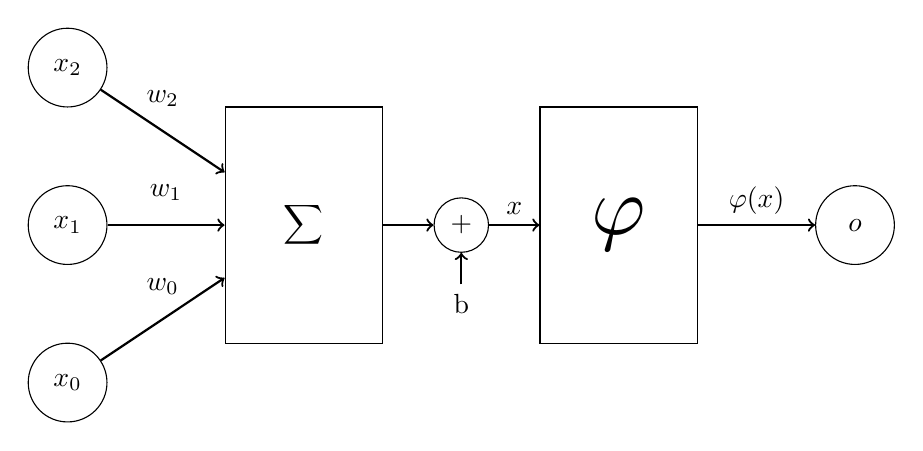
\begin{tikzpicture}

  \node[rectangle, draw=black, minimum size=2cm,minimum height=3cm] (sum) at (3, 0) {$\displaystyle\sum$};

  \foreach\name in {0,1,2}{
      \pgfmathsetmacro\y{2*\name-2}
  	\node[circle, draw=black,minimum size=1cm] (input\name) at (0, \y) {$x_{\name}$};
      \draw[thick,->] (input\name) to node[yshift=5pt,above] {$w_{\name}$} (sum);
  }

  \node[rectangle, draw=black, minimum size=2cm,minimum height=3cm] (phi) at (7, 0) {};
  \node[scale=3] (phisym) at (phi.center) {$\displaystyle\varphi$};

  \node (bias) at (5, -1) {b};
  \node[circle, draw=black] (sumb) at (5, 0) {$+$};
  \draw[thick,->] (sum.east) -- (sumb.west);
  \draw[thick,->] (bias.north) -- (sumb.south);
  \draw[thick,->] (sumb.east) -- node[above] {$x$} (phi.west);
  \node[circle,draw=black,minimum size=1cm] (out) at (10,0) {$o$};
  \draw[thick,->] (phi.east) -- node[above] {$\varphi(x)$} (out.west);
  \end{tikzpicture}
\end{document}


  }
\caption{Modélisation d'un neurone artificiel.}
\label{fig:neurone}
\end{figure}

\begin{figure}
  \begin{subfigure}[b]{0.5\textwidth}
    \includegraphics[width=\textwidth]{activations}
    \caption{Fonctions d'activation saturantes.}
    \label{fig:activations}
  \end{subfigure}
\begin{subfigure}[b]{0.5\textwidth}
  \includegraphics[width=\textwidth]{rectifiers}
  \caption{Fonctions d'activation non-saturantes.}
  \label{fig:rectifiers}
\end{subfigure}
\caption{Exemples de fonctions d'activation.}
\label{fig:activations}
\end{figure}

\begin{figure}
  \begin{subfigure}[b]{0.5\textwidth}
    \resizebox{\textwidth}{!}{
    \documentclass{standalone}
\usepackage[utf8]{inputenc}
\usepackage[T1]{fontenc}
\usepackage{tikz}
\input{../CommandesPerso.tex}
\begin{document}
  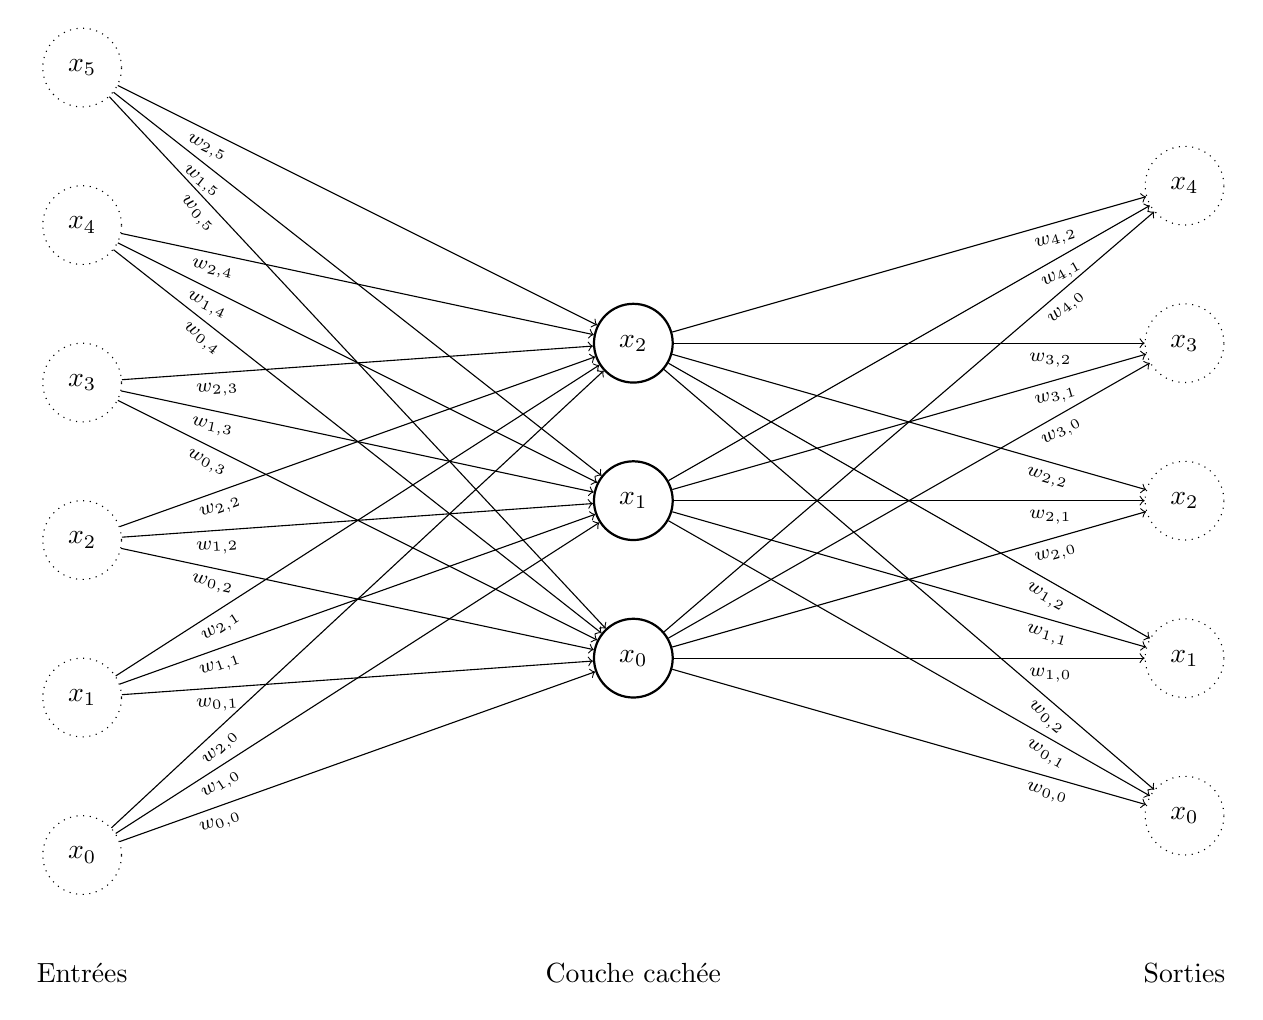
\begin{tikzpicture}
  \foreach\name in {0,1,2,3,4}{
      \pgfmathsetmacro\y{2*\name-3}
  	\node[circle, dotted,draw=black,minimum size=1cm] (output\name) at (7, \y) {$x_{\name}$};
  %    \draw[thick,->] (input\name) to node[yshift=5pt,above] {$w_{\name}$} (sum);
  }

  \foreach\name in {0,1,2}{
      \pgfmathsetmacro\y{2*\name-1}
  	\node[circle, thick,draw=black,minimum size=1cm] (hidden\name) at (0, \y) {$x_{\name}$};
      \foreach\oname in {0,1,2,3,4}{
      \draw[->] (hidden\name) to node[near end, sloped,pos=0.8,below] {\scriptsize $w_{\oname,\name}$} (output\oname);
      }
  }

  \node at (-7, -5) {Entrées};
  \node at (0, -5) {Couche cachée};
  \node at (7, -5) {Sorties};

  \foreach\name in {0,1,2,3,4,5}{
      \pgfmathsetmacro\y{2*\name-3.5}
  	\node[circle, dotted, draw=black,minimum size=1cm] (input\name) at (-7, \y) {$x_{\name}$};
      \foreach\hname in {0,1,2}{
      \draw[->] (input\name) to node[near end, sloped,pos=0.2,below] {\scriptsize $w_{\hname,\name}$} (hidden\hname);
      }
  }
  \end{tikzpicture}
\end{document}

    }
  \caption{Perceptron à une couche cachée.}
  \end{subfigure}%
  \begin{subfigure}[b]{0.5\textwidth}
    \resizebox{\textwidth}{!}{
    \documentclass{standalone}
\usepackage[utf8]{inputenc}
\usepackage[T1]{fontenc}
\usepackage{tikz}
\usepackage{ifthen}
\input{../CommandesPerso.tex}
\begin{document}

    \begin{tikzpicture}

    \newcommand\drawlayer[7]{%{nombre de neurones}{position en x}{symbole}{nom de la couche}{couche précédente}{n couche précédente}{style}
      \foreach\name in {0,...,#1}{
        \pgfmathsetmacro\y{2*(\name-#1/2)}
      	\node[circle,#7,draw=black,minimum size=1cm] (#4_\name) at (#2, \y) {$#3_{\name}$};
          \ifthenelse{\equal{#5}{}}{}{
		\foreach\oname in {0,...,#6}{
	            {\draw[->] (#5_\oname) to (#4_\name);}
         	 }
      	  }
      }
    }

    \drawlayer{5}{0}{x}{input}{}{}{dotted}
    \drawlayer{3}{4}{h^1}{hidden1}{input}{5}{thick}
    \drawlayer{4}{8}{h^2}{hidden2}{hidden1}{3}{thick}
    \drawlayer{3}{12}{h^3}{hidden3}{hidden2}{4}{thick}
    \drawlayer{3}{16}{y}{output}{hidden3}{3}{dotted}

    \node at (0,-6.5) {Entrées};
    \node at (8,-6.5) {Couches cachées};
    \node at (16,-6.5) {Sorties};

    \end{tikzpicture}

\end{document}


    }
  \caption{Perceptron multi-couches.}
  \end{subfigure}
  \caption{Perceptron à une et plusieurs couches. Les entrées et sorties peuvent être de dimensions variables et sont représentées comme des neurones.}
  \label{fig:perceptron}
\end{figure}

La définition formelle d'un neurone artificiel a été introduite par McCulloch et Pitts~\cite{lettvin_what_1959} en 1959. Un neurone doté d'une fonction de transfert $\varphi$ opère sur un ensemble de $n$ neurones d'entrée émettant chacun une valeur $x_1\dots{}x_n$, auxquelles il est connecté par des synapses de poids $w_i$. La valeur d'entrée $x$ du neurone correspond à la somme pondérée des signaux d'entrée. Le neurone émet ensuite l'image $z = \varphi(x)$ de ce signal par sa fonction de transfert. Le schéma de la~\cref{fig:neurone} décrit ce procédé. L'activation en sortie d'un neurone s'obtient donc par la formule
$$z = \varphi\left(\sum_{i=1}^n w_i x_i + b\right)~.$$

Plusieurs neurones connectés les uns aux autres forment un graphe orienté et pondéré. Un réseau de neurones à propagation avant désigne un graphe neuronal acyclique. En pratique, on considère des graphes multipartis que l'on peut alors représenter par \fg couches \og{}. Dans le cas d'un perceptron à couches multiples, les valeurs du signal d'entrée sont placées dans une couche d'entrée et les signaux de sortie envoyés dans une couche de sortie. La ou les couches de neurones réellement optimisables sont nommées \og couches cachées \fg{} et font l'interface entre l'entrée et la sortie. Le perceptron multi-couches à une et plusieurs couches cachées sont illustrés dans la~\cref{fig:perceptron}.

La fonction d'activation des neurones peut prendre de nombreuses formes. Il est \emph{a minima} nécessaire que celle-ci soit non-linéaire, sans quoi elle rend le perceptron multi-couches équivalent au perceptron simple, et presque partout différentiable afin de pouvoir appliquer l'algorithme de rétropropagation du gradient. La fonction d'activation est en outre généralement choisie monotone croissante et de dérivée monotone croissante. La~\cref{fig:activations} illustre plusieurs activations communément utilisées dans les réseaux de neurones artificiels profonds\,:
\begin{itemize}
  \item La \textbf{sigmoïde}, ou fonction logistique\,: $\sigma(x) = \frac{1}{1 + e^{-x}}$.
  \item La fonction \textbf{tangente hyperbolique}\,: $\tanh(x) = \frac{1 - e^{-2x}}{1 + e^{-2x}}$.
  \item La \textbf{marche de Heavyside}\,: $H(x) = 0 \text{ si } x < 0 \text{ et } 1 \text{ si } x \geq 0$.
  \item La fonction \textbf{\gls{ReLU}}\,: $ReLU(x) = max(0,x)$.
  \item La fonction \textbf{SoftPlus}\,: $s(x) = ln(1 + e^x)$.
\end{itemize}

La fonction sigmoïde, bien que populaire à l'origine, est une fonction saturante qui souffre de gradients évanescents. Ce problème n'est pas circonscrit à la sigmoïde et est particulièrement pregnant dans le cas des réseaux de neurones récurrents~\cite{hochreiter_gradient_2001}. L'accumulation de couches dans un réseau fait que la rétropropagation du gradient est similaire à une suite géométrique. Le produit cumulé de $n$ gradients dans des fonctions d'activation à tendance contractante produit un $n+1$ gradient plus faible que le précédent, et ainsi de suite. À l'inverse, il est possible d'avoir des gradients explosifs. Ce problème est empiré dans le cas des fonctions saturants comme la sigmoïde ou la tangente hyperbolique car leurs gradients sont nécessairement dans $[0,1]$. L'utilisation de la sigmoïde ou la tangente hyperbolique a varié dans la littérature. LeCun~\cite{lecun_efficient_1998} recommande d'utiliser la fonction hyperbolique modifiée $f(x) = 1,7159 tanh(\frac{2}{3} x)$, notamment car celle-ci est bornée par $[-1,1]$ et centrée en 0, ce qui est adapté au travail sur des données normalisées à moyenne nulle et variance unitaire.

La marche de Heavyside, tout comme la fonction $signe$, a des gradients nuls presque partout, sa dérivée étant l'impulsion de Dirac $\delta$.

Pour limiter les gradients évanescents, des fonctions non-linéaires non-saturantes sont désormais majoritairement utilisées dans la littérature. Glorot, Bordes et Bengio~\cite{glorot_deep_2011} ont ainsi proposé d'utiliser la fonction \gls{ReLU}, introduite précédemment pour les \gls{DBN}~\cite{nair_rectified_2010}, et la fonction SoftPlus pour les réseaux de neurones artificiels de toutes sortes. Leurs travaux aboutissent à trois conclusions importantes. Tout d'abord, les fonctions d'activation non-linéaire obtiennent généralement de meilleures performances que les réseaux utilisant $tanh$. Ensuite, les réseaux entraînés avec \gls{ReLU} ne nécessitent pas de pré-apprentissage non-supervisé couche par couche, ce qui accélère grandement les temps d'entraînement. Enfin, ces modèles sont plus parcimonieux que leurs équivalents usuels. En outre, la fonction \gls{ReLU} est simple à implémenter et rapide à calculer, ce qui a contribué à sa popularisation rapide dans la communauté.

Plusieurs variantes ont dès lors été proposées autour des fonctions linéaires rectifiées, notamment une version paramétrique dont la partie négative est non-saturante, mais linéaire de pente $\alpha$ fixée par l'utilisateur (\emph{Leaky ReLU}~\cite{maas_rectifier_2013}) ou optimisable (\gls{PReLU}~\cite{he_delving_2015}). Une version similaire mais continue a également été proposée sous la forme des \gls{ELU}~\cite{clevert_fast_2015}. Plus récemment, une recherche automatique quasi-exhaustive sur une variété de fonctions d'activation possibles a permis de proposer la \emph{Swish}~\cite{ramachandran_searching_2018}, non-linéaire non-saturante mais ayant la particularité d'être non-monotone. Ces variantes sont illustrées dans la~\cref{fig:rectifiers} et leur formule est donnée ci-dessous\,:
\begin{itemize}
  \item La fonction \textbf{\emph{Leaky ReLU}}\,: $LReLU_\alpha(x) = max(0,x) - \alpha max(0,-x)$, avec $\alpha$ un hyperparamètre.
  \item La fonction \textbf{\gls{PReLU}}\,: $PReLU(x, \alpha) = max(0,x) - \alpha max(0,-x)$, avec $\alpha$ optimisable.
  \item La fonction \textbf{\gls{ELU}}\,: $ELU_\alpha(x) = x \text{ si } x > 0 \text{ et } \alpha (exp(x) - 1) \text{ sinon}$.
  \item La fonction \textbf{\emph{Swish}}\,: $Swish_\beta(x) = x . \sigma(\beta x) = x . (1 + e^{-\beta x})^{-1}$.
\end{itemize}
% TODO : ref Oyallon sur les "bonnes" hypothèses pour la fonction d'activation

Le théorème d'approximation universelle~\cite{cybenko_approximation_1989,hornik_approximation_1991} indique que l'ensemble des fonctions engendrées par les perceptrons est dense dans l'ensemble des fonctions continues par morceaux sur des compacts. Autrement dit, toute fonction $f : E \rightarrow \mathbb{R}^m$ avec $E = \bigcup\limits_{k} C_k$ une union de compacts de $\mathbb{R}^n$ continue sur chaque compact est approximable à une précision $\epsilon$ arbitraire par un perceptron. On peut voir deux limitations à ce résultat. Le premier concerne la nature de la fonction d'activation. Le théorème généralisé par Hornik s'applique à tous les perceptrons sur lesquels on applique une fonction d'activation monotone non-constante et bornée, cela couvre les fonctions saturantes $tanh$ et sigmoide, mais exclut les fonctions linéaires rectifiées comme \gls{ReLU}. Ce problème a cependant été levé par Sonoda et Murata~\cite{sonoda_neural_2017}, qui ont montré que des réseaux munis de fonctions d'activation non-bornées satisfaient tout de même le théorème d'approximation universelle


La deuxième limitation porte quant à elle sur la nature même du théorème. Celui-ci ne donne qu'une garantie purement théorique concernant l'existence d'un ensemble de paramètres permettant l'approximation à la précision voulue. Il ne donne pas de bornes sur le nombre de neurones nécessaire, ni de méthode de construction. Ainsi, il n'y aucune certitude que les poids puissent être obtenus par descente de gradient, ni d'indication sur l'architecture à choisir. En particulier, le théorème vaut pour des réseaux superficiels à une seule couche. Pourtant, le consensus scientifique dans la communauté tend à préférer des réseaux de plus en plus profonds. Ainsi, il a été démontré que des réseaux plus profonds demandent moins de poids et de neurones pour approximer des fonctions plus complexes~\cite{bianchini_complexity_2014,mhaskar_when_2017}. En particulier, la structure hiérarchique des réseaux multi-couches semble adapté à l'approximation de fonctions composées en contournant la malédiction de la dimension~\cite{poggio_why_2017}. Toutefois, cela augmente également le nombre d'hyperparamètres à régler pour définir l'architecture. L'absence de méthode systématique de construction des architectures de réseau profond conduit donc à l'utilisation intensive de la méthode essai-erreur ou à des méthodes de méta-apprentissage~\cite{zoph_neural_2016}.

\subsection{Réseaux de neurones convolutifs profonds}

L'idée de partager des poids pour réaliser de façon dense la même opération locale sur toute l'image remonte au Neocognitron~\cite{fukushima_neocognitron_1980}. L'idée d'utiliser des convolutions remonte à LeCun~\cite{lecun_gradient-based_1998}. Le produit de convolution entre deux fonctions $f$ et $g$ est habituellement noté $f * g$ s'obtient par la formule suivante\,:
$$(f * g)(x) = \int_{-\infty}^{+\infty} f(t)g(x-t)\diff t$$

Ce produit est commutatif et bilinéaire.

L'intérêt principal du produit de convolution est son lien fondamental avec la transformée de Fourier~\cite{fourier_propagation_1822}. En effet, en notant $\fourier$ la transformation de Fourier, alors\,:
$$\fourier(f \ast g) = \fourier (f)\fourier (g)~.$$


Les convolutions avaient déjà été utilisées de nombreuses fois, en particulier compte-tenu des résultats de Fourier en analyse harmonique~\cite{fourier_propagation_1822}. En partiuclier, la convolution discrète permet de réaliser des calculs de gradients, utilisés dans les \gls{SIFT}~\cite{lowe_object_1999} et \gls{HOG}~\cite{dalal_histograms_2005}. Les filtres convolutifs sont également à la base de la théorie des ondelettes~\cite{mallat_exploration_2001}, utilisés notamment dans le format compressé \gls{JPEG}~\cite{daubechies_ten_1992}. Les filtres de Gabor en particulier ont trouvé de nombreuses applications comme caractéristique image~\cite{pati_word_2008}. Incidemment, plusieurs travaux de neurosciences ont mis en évidence la proximité entre le modèle de filtre de Gabor et les réponses des cellules du cortex visuel chez les mammifères, notamment le chat~\cite{marcelja_mathematical_1980,jones_evaluation_1987}. La~\cref{fig:convolution_exemples} illustre le résultat de filtrages par divers noyaux de convolution classiques.

L'idée de LeCun~\cite{lecun_gradient-based_1998} est de remplacer les premières couches d'un réseau de neurones par des couches convolutives. Les neurones seront donc regroupés localement et calculeront chacun une convolution sur une partie de l'image. Pour simplifier le modèle, les poids seront partagés, c'est-à-dire que tous les neurones calculeront la même convolution. Plusieurs convolutions pourront toutefois être calculées en parallèle. Les noyaux de convolution étant optimisés durant l'apprentissage, l'apprentissage par représentation va donc se faire naturellement dans le domaine image avec des opérateurs adaptés. Incidemment, il s'avère qu'en pratique, la première couche convolutive tend à approximer des filtres de Gabor~\cite{yosinski_how_2014}.

\subsubsection{Convolution}


\begin{figure}
  \foreach \picpath\piclegend in {nobu/Image originale,nobu_gabor/Filtre de Gabor,nobu_sobel/Filtre de Sobel~\cite{sobel_isotropic_2014},nobu_frangi/Filtre de Frangi~\cite{frangi_multiscale_1998}}{%
  \begin{subfigure}{0.25\textwidth}
    \includegraphics[width=\textwidth]{\picpath}
    \caption*{\piclegend}
  \end{subfigure}%
  }
  \caption{Exemples de filtrages par différents noyaux de convolution.}
  \label{fig:convolution_exemples}
\end{figure}


\begin{figure}
  \foreach \picpath\piclegend in {no_padding_no_strides_00/Convolution,padding_strides_00/Convolution avec pas et padding,dilation_00/Convolution à trous,no_padding_no_strides_transposed_00/Déconvolution}{%
\begin{subfigure}[b]{0.25\textwidth}
  \includegraphics[width=\textwidth]{\picpath}
  \caption*{\piclegend}
\end{subfigure}%
}
\caption{Opérateur de convolution et variantes sur une image (figures extraites de~\cite{dumoulin_guide_2016}).}
\label{fig:convolution}
\end{figure}

Dans le cas discret, le produit de convolution se réécrit\,:
$$(f * g)[n] = \sum_{k=-\infty}^{+\infty} f[n]g[k-n]$$

Cette formulation s'intéresse toutefois aux signaux 1D, tandis que les images sont des signaux 2D par nature. La convolution discrète peut toutefois s'écrire sans problème pour des fonctions multivariées. Si l'on note $I : \llbracket 1;w \rrbracket \times \llbracket 1;h \rrbracket \rightarrow \mathbb{R}$ la fonction modélisant une image $I$ de dimensions $w\times{}h$ et $K\,: \llbracket 1;k_w \rrbracket \times \llbracket 1;k_h \rrbracket \rightarrow \mathbb{R}$ le \emph{noyau} de convolution de dimension $p \times q$, alors on peut définir le filtre $\mathcal{K}$ tel que\,:
$$\mathcal{K}(I)(m,n) = \sum_{i=-p}^{+p} \sum_{i=-q}^{+q} I[m - i, n - j] \cdot k[i, j]~,$$
avec $p = \frac{k_w-1}{2}$ et $q = \frac{k_h-1}{2}$. Ce calcul est illustré dans la~\cref{fig:convolution}.

Cette formule souffre néanmoins d'une inconnue lorsque l'opérateur agit sur les bords de l'image, puis que les valeurs de $I$ sont alors manquantes. En règle générale, soit on ne calcule pas ces valeurs, auxquel cas la taille de l'image résultante est diminuée par rapport à celle de l'image initiale, soit on ajoute un nombre de zéros égal à la moitié de la taille du noyau de convolution dans chaque direction (\emph{padding}).

En pratique, une couche convolutive d'un réseau de neurones est paramétrée par\,:
\begin{itemize}
  \item La taille $k$ des noyaux de convolution, généralement la même dans tous les dimensions,
  \item Le nombre $C$ de convolutions parallèles, qui définit le nombre de cartes d'activations en sortie de couche,
  \item Le pas $s$ de la convolution,
  \item Le \emph{padding} $p$.
\end{itemize}

Conventionnellement, on représente les cartes d'activation des neurones, ou cartes de caractéristiques, sous la forme de tenseurs de dimension 3 $(C, W, H)$ avec $C$ le nombre de canaux, également appelé nombre de plans de convolutions, $W$ la largeur et $H$ la hauteur des cartes.

Une couche convolutive va donc combiner les $n_{in}$ cartes d'activation d'entrée avec le $j$\ieme{} noyau de convolution $K_j$\,:
$$\forall j \in \llbracket 1;n_{out} \rrbracket,~~~o_j = b_j + \sum_{i=1}^{n_{in}} K(z_i)~,$$ c'est-à-dire\,:
$$\forall j \in \llbracket 1;n_{out} \rrbracket,~~~o_j(m, n) = b_j + \sum_{i=1}^{n_{in}} \sum_{p=-\frac{k-1}{2}}^{+\frac{k-1}{2}} \sum_{q=-\frac{k-1}{2}}^{+\frac{k-1}{2}} z_i(m - p, n - q) \cdot k_j(p, q)$$

Une convolution transforme donc un tenseur $(C_{in}, W_{in}, H_{in})$ en tenseur $(C_{out}, W_{out}, H_{out})$ avec les dimensions spatiales se calculant par\,:
$$out = \left\lfloor \frac{in - kernel + 2\cdot{}padding}{stride}\right\rfloor + 1~.$$

\todo[inline]{formule pour la convolution avec stride}


\paragraph{Convolution à trous}

Avec un facteur de dilatation $d$\,:
$$\forall j \in \llbracket 1;n_{out} \rrbracket,~~~o_j(m, n) = b_j + \sum_{i=1}^{n_{in}} \sum_{p=-\frac{k-1}{2}}^{+\frac{k-1}{2}} \sum_{q=-\frac{k-1}{2}}^{+\frac{k-1}{2}} z_i(m - dp, n - dq) \cdot k_j(p, q)$$

À trous\,:
$$out = \left\lfloor \frac{in - kernel - (kernel -1)(dilation - 1) + 2\cdot{}padding}{stride}\right\rfloor + 1~.$$


\paragraph{Déconvolution}

$$out = (in - 1) \cdot stride + kernel - 2padding~.$$

\subsubsection{Échantillonnage}

\begin{figure}
  \resizebox{\textwidth}{!}{
  \documentclass{standalone}
\usepackage[utf8]{inputenc}
\usepackage[T1]{fontenc}
\usepackage{tikz}
\begin{document}
\definecolor{backcolor}{RGB}{228,188,45}
\definecolor{frontcolor}{RGB}{97,39,153}
\definecolor{idxcolor}{RGB}{39,89,149}
\definecolor{zerocolor}{RGB}{0,0,0}

\def \backcolor {backcolor!50!white}
\def \frontcolor {frontcolor!50!white}
\def \idxcolor {idxcolor!50!white}
\def \zerocolor {zerocolor!50!white}
\usetikzlibrary{patterns}
\begin{tikzpicture}[%%%%%%%%%%%%%%%%%%%%%%%%%%%%%%
        box/.style={rectangle,fill=\backcolor, minimum size=1cm},
        mbox/.style={rectangle,fill=\frontcolor, minimum size=1cm},
        zbox/.style={rectangle,fill=\zerocolor,fill=\backcolor!50!white,minimum size=1cm},
        ibox/.style={rectangle,fill=\idxcolor,minimum size=1cm},
    ]
% Main map

\node[box] at (-7.5,+1.5) {1.5};
\node[box] at (-7.5,+0.5) {2.0};
\node[mbox] at (-7.5,-0.5) {\textbf{2.3}};
\node[box] at (-7.5,-1.5) {2.2};

\node[box] at (-6.5,+1.5) {1.7};
\node[mbox] at (-6.5,+0.5) {\textbf{2.1}};
\node[box] at (-6.5,-0.5) {1.9};
\node[box] at (-6.5,-1.5) {2.1};

\node[box] at (-5.5,+1.5) {1.4};
\node[mbox] at (-5.5,+0.5) {\textbf{1.8}};
\node[box] at (-5.5,-0.5) {1.5};
\node[box] at (-5.5,-1.5) {1.6};

\node[box] at (-4.5,+1.5) {1.3};
\node[box] at (-4.5,+0.5) {1.6};
\node[box] at (-4.5,-0.5) {1.4};
\node[mbox] at (-4.5,-1.5) {\textbf{1.7}};

\draw[step=1,color=gray] (-8,-2) grid (-4,2);

\draw[->,ultra thick,bend left] (-3.5,0) to node[above] {maxpooling}  (-1.5,0);

% Pooled map
\node at (0, 2.5) {indices};
\node[ibox] at (-0.5,+1.75) {\footnotesize (1,1)};
\node[ibox] at (-0.5,+0.75) {\footnotesize (0,2)};
\node[ibox] at (+0.5,+1.75) {\footnotesize (2,1)};
\node[ibox] at (+0.5,+0.75) {\footnotesize (3,3)};
\draw[step=1,color=gray,shift={(0,0.25)}] (-1,0) grid (1,2);

\node[mbox] at (-0.5,-1.75) {\textbf{2.1}};
\node[mbox] at (-0.5,-0.75) {\textbf{2.3}};
\node[mbox] at (+0.5,-1.75) {\textbf{1.8}};
\node[mbox] at (+0.5,-0.75) {\textbf{1.7}};
\draw[step=1,color=gray,shift={(0,-0.25)}] (-1,0) grid (1,-2);
\node at (0, -2.5) {activations};

\draw[->,ultra thick,bend left] (1.5,0) to node[above] {unpooling}  (3.5,0);

% Unpooled map
\node[zbox] at (7.5,+1.5) {0};
\node[zbox] at (7.5,+0.5) {0};
\node[zbox] at (7.5,-0.5) {0};
\node[mbox] at (7.5,-1.5) {\textbf{1.7}};

\node[zbox] at (6.5,+1.5) {0};
\node[mbox] at (6.5,+0.5) {\textbf{1.8}};
\node[zbox] at (6.5,-0.5) {0};
\node[zbox] at (6.5,-1.5) {0};

\node[zbox] at (5.5,+1.5) {0};
\node[mbox] at (5.5,+0.5) {\textbf{2.1}};
\node[zbox] at (5.5,-0.5) {0};
\node[zbox] at (5.5,-1.5) {0};

\node[zbox] at (4.5,+1.5) {0};
\node[zbox] at (4.5,+0.5) {0};
\node[mbox] at (4.5,-0.5) {\textbf{2.3}};
\node[zbox] at (4.5,-1.5) {0};
\draw[step=1,color=gray] (8,-2) grid (4,2);
\end{tikzpicture}
\end{document}


  }
  \caption{Sous-échantillonnage et sur-échantillonnage par valeurs maximales en deux dimensions.}
  \label{fig:pooling}
\end{figure}

\paragraph{Sous-échantillonnage}

Afin de réduire la dimension des cartes d'activation dans le réseau, il est utile d'opérer à des sous-échantillonnages. Il s'agit généralement d'appliquer un filtre par fenêtre glissante non-recouvrante sur les données d'entrée. Ce filtre est en règle général l'opérateur $\max$ ou l'opérateur de moyenne sur une fenêtre de taille fixe.

Outre la réduction de dimension, l'intérêt de ces opérateurs est d'introduire une invariance aux déformations légères.

Par ailleurs, il est possible de réaliser un sous-échantillonnage adaptatif dans le cas du filtre moyen. Il est utilisé dans certains réseaux pour réduire brutalement la dimension des cartes d'activation lorsque l'on traite des images de taille arbitraire. Dans le cas contraire, les dimensions des couches entièrement connectées déterminent la taille des images d'entrée.
Max-pooling, average pooling, adaptative pooling

Les dimensions d'une carte d'activation en sortie d'un sous-échantillonnage sont\,:
$$out = \left\lfloor \frac{in - kernel}{stride}\right\rfloor + 1~.$$

\paragraph{Sur-échantillonnage}
Les dimensions d'une carte d'activation en sortie d'un sur-échantillonnage sont\,:
$$out = (in - 1) \cdot stride + kernel~.$$

\subsubsection{Normalisation}

Si la normalisation des données afin de faire travailler les modèles sur des distributions centrées et normalisées est une pratique ancienne, l'utilisation de couches de normalisation des activations au sein même des réseaux profonds est relativement récente. Le principe général de la normalisation est d'appliquer une transformation aux cartes d'activation afin de leur imposer des propriétés statistiques particulières pour améliorer les capacités d'apprentissage du modèle.

\citet{jarrett_what_2009} propose ainsi une normalisation locale du contraste des cartes d'activation après les couches convolutives en s'inspirant des modèles biologiques~\cite{pinto_why_2008}. Pour un tenseur de $N$ cartes d'activations $a_1,\dots,a_N$, les cartes normalisées $z_i$ s'obtiennent par d'abord par soustraction d'une valeur moyenne locale sur une fenêtre spatiale gaussienne\,:
$$b_i[x,y] = a_i[x,y] - \sum_{p,q} w_{p,q} \cdot a_i[x+p,j+q]$$ avec $w_pq$ une fenêtre gaussienne telle que $\sum_{p,q} w_{p,q} = 1$
puis par normalisation des amplitudes par l'écart-type pondéré des caractéristiques sur une fenêtre spatiale\,:
$$z_i[x,y] = b_i[x,y] / max(\operatorname{moy}(\sigma[x,y]), \sigma[x,y])$$ avec $\sigma[x,y] = \left(\sum_{p,q} w_{p,q} \cdot b_i^2[x+p,y+q] \right)^{\frac{1}{2}}$.

L'article séminal de~\citet{krizhevsky_imagenet_2012} introduit également une couche de normalisation locale, \emph{Local Response Normalization}, qui vient inhiber les activations des cartes d'activations adjacentes à celle d'un neurone fortement excité. Ce procédé inspiré de l'inhibition latérale existant dans les neurones biologiques permet d'améliorer la généralisation du modèle. Contrairement à la normalisation du contraste de \citet{jarrett_what_2009}, cette normalisation ne s'applique pas sur un voisinage spatial, mais sur les cartes d'activations filtrées voisines de celle considérée, dans la troisième direction du tenseur. Cette normalisation peut s'exprimer sous la forme d'un noyau s'appliquant aux cartes d'activation 2D. Pour un tenseur de $N$ cartes d'activations $a^1,\dots,a^N$, les cartes normalisées $z^i$ s'obtiennent par\,:
$$z^i[x,y] = \frac{a^i[x,y]}{\left(k + \alpha \sum_{j=max(0, i-n/2)}^{min(N-1, i+n/2)} (a^j[x,y])^2  \right)^\beta}~~.$$
avec $n$ la taille du voisinage à considérer (dans la direction des canaux). Il est possible d'envisager cette normalisation en considérant pour chaque position spatiale des cartes d'activation qu'il s'agit d'une normalisation de l'intensité du vecteur d'activation $(a[x,y]^1, a[x,y]^2, \dots, a[x,y]^N)$.

Toutefois, la normalisation des activations la plus courante est la normalisation par lot, ou \emph{Batch Normalization}~\cite{ioffe_batch_2015}. Ce procédé consiste à normaliser les moments statistiques des cartes d'activation plan par plan afin de les center et de leur conférence une variance unitaire. Il présuppose un entraînement en utilisant l'algorithme de descente de gradient stochastique par mini-lots. Pour un lot de taille $N$, le réseau opère à chaque itération sur un tenseur $(N, C, W, H)$. Si l'on considère les activations pour une couche donnée, alors il est possible de considérer pour chaque élément $n$ du lot les cartes d'activation $a^{(n)}_i, i \in \llbracket 1,C \rrbracket$. On peut alors normaliser ces activations par\,:
$$\hat{a}_i = \frac{a_i - \mu_i}{\sqrt{\sigma_i^2 + \epsilon}}$$.

Durant la phase d'apprentissage, $\mu$ et $\sigma$ sont calculés à la volée à partir du \emph{mini-batch}\,:
$$\mu_i = \frac{1}{N} \sum_{j=1}^N a_i^{(j)}~~\text{ et }~~\sigma_i = \frac{1}{N} \sum_{j=1}^N (a_i^{(j)} - \mu_i)$$

Afin de rendre les calculs en phase d'inférence indépendants de la taille du \emph{batch}, les moments estimés durant la phase d'apprentissage sont conservés en mémoire et fixés lors de l'évaluation. La normalisation par lot est généralement suivie d'une transformée affine $z_i = \alpha \hat{a}_i + \beta$.

Cette normalisation possède une propriété critique pour l'optimisation de réseaux très profonds\,: elle garantit le flux du gradient couche après couche en maintenant les amplitudes des activations constantes. Les activations ne peuvent ni être trop élevée, ni trop faibles, ce qui assure la stabilité numérique de l'ensemble du réseau. En outre, la normalisation des représentations permet de limiter l'impact de perturbations non sémantiquement pertienentes dans le calcul des caractéristiques. En pratique, l'utilisation de la \emph{batch normalization} permet d'améliorer les performances de classification des modèles et accélère significativement leur vitesse de convergence. Cette normalisation se retrouve dans la grande majorité des architectures de réseaux profonds conçues après sa publication.

\subsection{Entraînement des réseaux de neurones}

Un autre inconvénient au théorème d'approximation universelle est que même si l'architecture était connue, celui-ci ne donne aucune méthode pour trouver les valeurs des paramètres. En particulier, l'algorithme de rétropropagation du gradient~\cite{werbos_beyond_1975,rumelhart_learning_1986,lecun_learning_1986} décrit ci-après se base sur une méthode de descente de gradient. Toutefois, rien ne garantit que les poids optimaux dont l'existence est assurée par le théorème d'approximation universelle ne soit trouvables par cet algorithme.

L'algorithme de rétropropagation du gradient se fonde sur la règle de dérivation en chaîne, c'est-à-dire le théorème de dérivation des fonctions composées~\cite{lhospital_analyse_1716,lagrange_theorie_1797}\,:
\begin{theorem}
Soient $f$ et $g$ deux fonctions telles que $f : I \rightarrow J \subset \mathbb{R}$ et $g : J \rightarrow \mathbb{R}$. Soit $x \in I$ tel que $f$ admet une dérivée en $x$. Alors, la fonction composée $h = g \circ f : I \rightarrow \mathbb{R}$ admet une dérivée en $x$ de valeur :
$$h'(x) = (g \circ f)'(x) = f'(x) \times g'(f(x))~.$$

Si $f$ et $g$ sont dérivables respectivement sur $I$ et $J$, alors\,:
$$(g \circ f)' = f' \times (g' \circ f)~.$$

ou encore, en utilisant la notation de Leibniz, avec $z = g(y)$ et $y = f(x)$:
$$\frac{\diff z}{\diff x} = \frac{\diff z}{\diff y} \times \frac{\diff y}{\diff x}~.$$
\end{theorem}

Ce théorème s'étend aux dérivées partielles de fonctions à valeurs dans $\mathbb{R}^n$.

Dans le cas des réseaux profondes, la propagation avant des activations se fait par la formule suivante\,:
$$z_j^{k+1} = \varphi\left(\sum_{i=1}^n w^k_{i,j} \cdot z^k_i + b^k_j\right)$$
avec $\varphi$ la fonction d'activation, $w_{i,j}$ le poids de la connexion, $b_i$ le biais et $k$ le numéro de la couche.

En connaissant l'erreur $e^{k+1}$, c'est-à-dire le gradient pour la couche $k+1$, alors\,:

$$e^k_j = \sum_{i=1}^N w^k_{i,j} e^{k+1}_j  \varphi'\left(\sum_{i=1}^n w^k_{i,j} \cdot z^k_i + b^k_j\right)$$

Pour diminuer l'erreur, il est nécessaire de mettre à jour les poids $w^k$ dans la direction opposée au gradient $\frac{\diff e}{\diff w^k}$. Or, grâce à la règle de la dérivation en chaîne\,:
$$\frac{\diff e}{\diff w^k} = \frac{\diff e}{\diff z^k} \times \frac{\diff z^k}{\diff w^k}$$.

Il est donc possible de calculer la mise à jour des poids en rétro-propageant la valeur du gradient d'une couche à la précédente.

On peut alors utiliser l'algorithme de descente de gradient~\cite{cauchy_comptes_1847} afin de minimiser l'erreur totale en mettant à jour les poids. Cet algorithme, dit de la plus forte pente, permet d'approcher des minima locaux d'une fonction $f$ arbitraire en cherchant ses points stationnaires, c'est-à-dire les points où le gradient de $f$ s'annule. L'algorithme repose sur l'idée que $f$ décroît le plus rapidement dans la direction opposée à son gradient et fonctionne de la façon suivante\,:

\begin{theorem}
  Soit $f : \mathbb{R}^n \rightarrow \mathbb{R}$ une fonction différentiable et $\nabla f$ son gradient. Soit $x_0 \in \mathbb{R}^n$ un point initial, $\epsilon > 0$ le seuil de tolérance de l'algorithme et $\alpha > 0$ le pas de la descente. On définit alors la suite $(x_i)_{i \ge 0} \in \mathbb{R}^\mathbb{N}$ telle que\,:
  $$x_{i+1} = x_i - \alpha \nabla f(x_i)~.$$
  L'algorithme s'arrête lorsque $\nabla f(x_i) \le \epsilon$.
\end{theorem}

Dans le cas des réseaux de neurones, la fonction $f$ correspond à l'erreur totale du modèle sur l'ensemble du jeu de données d'entraînement $\Omega$. Ainsi, pour un modèle paramétré par ses poids $W$ et de fonction objectif $E$, on cherche à mettre à jour les poids du réseau dans la direction opposée du gradient par rapport à ces mêmes poids $\nabla_W E(W, \Omega)$.

\begin{theorem}
  \begin{enumerate}
    \item Initialiser aléatoirement les poids $W$.
    \item Calculer $\nabla_W E(W, \Omega)$ à partir de l'erreur sur chaque échantillon.
    \item Tant que $\nabla_W E(W, \Omega) > \epsilon$\,:
      \begin{itemize}
          \item $W = W - \nabla_W E(W, \Omega)$
      \end{itemize}
  \end{enumerate}
\end{theorem}

 Cependant, le cardinal de $\Omega$ peut être très grand en pratique, les bases de données d'apprentissage pouvant contenir des milliers, voire des millions d'exemple. Par conséquent, il est généralement nécessaire d'utiliser une variante en ligne de l'algorithme de gradient, l'algorithme de descente de gradient \emph{stochastique}, qui réalise la mise à jour des poids pour chaque exemple, en approximant l'erreur moyenne à partir de l'erreur sur un seul échantillon, c'est-à-dire\,:
\begin{theorem}
  \begin{enumerate}
    \item Initialiser aléatoirement les poids $W$.
    \item Tant que le critère d'arrêt n'est pas atteint\,:
      \begin{itemize}
          \item Tirer aléatoirement un exemple d'apprentissage $\omega \in \Omega$
          \item $W = W - \nabla_W E(W, \omega)$
      \end{itemize}
  \end{enumerate}
L'algorithme s'arrête lorsque le critère d'arrêt est vérifié, généralement lorsqu'un nombre d'itérations prédéfini est atteint.
\end{theorem}

L'inconvénient de l'algorithme de descente de gradient stochastique est que l'approximation du gradient $\nabla_W E(W, \omega)$ est très bruitée et peut changer fortement de direction entre deux itérations successives. Afin de stabiliser la convergence, on utilise le plus souvent l'algorithme de descente de gradient stochastique \emph{par mini-lots}, également appelés \emph{mini-batches}. On approxime alors le gradient global non pas à partir d'un échantillon, mais à partir de la moyenne sur un nombre $k$ d'échantillons, qui forment un mini-lot ou \emph{mini-batch}\,:
\begin{theorem}
  \begin{enumerate}
    \item Initialiser aléatoirement les poids $W$.
    \item Tant que le critère d'arrêt n'est pas atteint\,:
      \begin{itemize}
          \item Tirer aléatoirement $k$ exemples d'apprentissage $(\omega_1,\dots,\omega_k) \in \Omega^k$
          \item $W = W - \frac{1}{k} \sum_{i=1}^k \nabla_W E(W, \omega_i)$
      \end{itemize}
  \end{enumerate}
L'algorithme s'arrête lorsque le critère d'arrêt est vérifié, généralement lorsqu'un nombre d'itérations prédéfini est atteint.
\end{theorem}

Il est important de noter que l'algorithme de descente de gradient ne dispose d'une convergence garantie que dans le cas où la fonction $f$ est convexe, ce qui n'est jamais le cas en pratique pour des réseaux profonds. Des variantes de la descente de gradient ont été proposées pour améliorer ses propriétés de convergence. En particulier, le pas de la descente $\alpha$ joue un rôle important dans l'optimisation des réseaux de neurones profonds. Appelé généralement taux d'apprentissage, $\alpha$ contrôle à l'amplitude des mises à jour des poids du modèle. Si $\alpha$ est très élevé, les mises à jour seront très grande et la convergence très instable. Si $\alpha$ est très faible, la convergence peut être très lente voire se bloquer dans des minima locaux. La plupart des variantes de la descente de gradient stochastique utilisent des politiques particulières pour la mise à jour des poids. Des méthodes dites de \og moment \fg, inspirées du moment cinétique en mécanique, permettent notamment de faire conserver au gradient une partie de sa vélocité des itérations précédentes pour limiter les oscillations le long des courbes de niveaux de la fonction~\cite{qian_momentum_1999,nesterov_method_1983}. \citet{sutskever_importance_2013-1} ont notamment montré que l'utilisation d'une descente de gradient stochastique à moment permet d'améliorer les performances finales du modèle, y compris dans le cas d'une poids initiaux mal choisis. \citet{polyak_acceleration_1992} propose par ailleurs d'utiliser le gradient moyennée sur les $n$ dernières itérations pour la mise à jour des poids, ce qui correspond à une forme de mini-lot asynchrone.

Une autre source d'amélioration proposée réside dans la politique du choix de $\alpha$. En effet, rien ne contraint $\alpha$ à être fixé dans l'algorithme de descente de gradient. Il est possible de l'ajuster manuellement au cours de l'apprentissage, par exemple en commençant avec un taux d'apprentissage élevé au début, puis en le multipliant par un ratio $\gamma < 1$ à intervalles réguliers. \citet{bottou_stochastic_2012} recommande ainsi de la descente de gradient stochastique moyennée couplée avec une évolution de $\alpha$ suivant la relation $\alpha_{i+1} = \alpha_0 (1 + \gamma \cdot i)^{-1}$. Plus récemment, \citet{loshchilov_sgdr_2016} ont proposé une méthode à base de recuit simulé. Toutefois, cela nécessite une intervention manuelle dans la mesure où il est nécessaire de configurer un certain nombre d'hyperparamètres au préalable. Plusieurs travaux se sont donc penchés sur des méthodes à moment dites adaptatives, dans lesquelles le taux d'apprentissage $\alpha$ est automatiquement ajusté selon une heuristique~\cite{duchi_adaptive_2011,tielman_lecture_2012,zeiler_adadelta_2012,kingma_adam_2014}.

De façon orthogonale à l'algorithme de descente de gradient utilisé, un point crucial dans l'optimisation des réseaux profonds réside dans le choix des poids initiaux. L'\emph{initialisation} de ceux-ci conditionne également la capacité de la descente gradient à converger vers un optimal de bonne qualité. Si, comme nous avons pu le voir, les méthodes de pré-entraînement non-supervisées ont été plebiscitées par le passé~\cite{hinton_fast_2006,bengio_greedy_2007}, les réseaux sont dorénavant directement entraînés de façon supervisée. L'idée principale concernant l'initialisation des poids consiste à leur assigner des valeurs aléatoires qui limitent l'explosion ou l'évanescence des gradients. \citet{glorot_understanding_2010-1} propose ainsi une méthode d'initialisation permettant d'obtenir des activations initiales normalement distribuées, ce qui facilite l'apprentissage en garantissant un flot raisonnable des gradients. Cette approche a été reprise et adaptée par la suite pour les fonctions d'activation de type \gls{ReLU}~\cite{he_delving_2015}. Dans la même veine, \citet{saxe_exact_2013} ont proposé d'initialiser les noyaux de convolution profonds avec des matrices aléatoires orthogonales afin d'une part de conserver la norme des activations d'une couche à l'autre et d'autre part de décorreller entre eux les filtres initiaux.

\todo[inline]{tips and tricks sur la SGD (Bottou, LeCun, Bengio, Schmidhuber)}
Mélanger les données
Normaliser les données
SGD avec moment
Évolution du learning rate
Taille des batch
etc.

Il est important de noter que la descente de gradient minimise l'erreur sur le jeu d'entraînement, tandis que l'erreur qui nous intéresse réellement est celle de généralisation. Toutefois, nous n'avons pas accès à cette erreur et devons donc nous contenter de celle disponible. Cela conduit toutefois à un phénomène de surapprentissage, c'est-à-dire que le modèle va apprendre et intégrer des connaissances biaisées liées aux échantillons du jeu d'entraînement, mais dont les propriétés ne se généralisent pas aux données réelles. Par exemple, un modèle devant discriminer entre des images de chats et des images de chiens entraîné sur des photos de chats prises majoritairement de jour et des photos de chiens prises majoritairement de nuit risquerait d'apprendre des caractéristiques liées à l'illumination plutôt qu'à l'espèce de l'animal.
Pour limiter ce phénomène de surapprentissage, il est nécessaire de faire intervenir des techniques de \emph{régularisation}. Celles-ci permettent de contrebalancer le fait que la fonction objectif à optimiser n'est connue que sur un sous-ensemble restreint et nécessairement biaisé de l'ensemble des observations du monde. Une première méthode consiste à imposer une contrainte sur l'amplitude des poids des connexions du réseau. Cette méthode, appelée \emph{weight decay}, ou dégradation des pondérations, ajoute une pénalité au terme d'erreur global dépend de la norme des poids. Ainsi, la fonction de coût totale devient\,:
$$E_{totale} = E_{coût} + \lambda \sum_{w \in W} w^2~~.$$
~\citet{krogh_simple_1991} ont montré que cette simple pénalité permet de réduire l'erreur de généralisation du modèle.

Plus récemment, le Dropout~\cite{srivastava_dropout_2014} a été proposé comme méthode de régularisation pour lutter contre le surapprentissage. Les réseaux de neurones contenant de nombreux paramètres, l'idée est d'aléatoirement éteindre des neurones de certaines couches à chaque itération de la phase d'apprentissage. Toutes les connexions liées aux neurones éteints sont alors neutralisées avec une probabilité $p$ et seuls les poids du réseau réduit sont mis à jour lors de la descente de gradient pour cette itération. Lors de la phase d'inférence, toutes les activations liées à ces neurones sont pondérées par $p$ afin de conserver les amplitudes totales constantes. Les n\oe{}uds du réseau ne voient ainsi qu'une partie du jeu de données, ce qui force les représentations à contenir de la redondance pour conserver leur pouvoir discriminant. Les signaux faibles liés au biais intrinsèque du jeu de données ne peuvent alors être modélisés, palliant ainsi aux problèmes de surapprentissage. Une autre façon d'envisager le Dropout est de considérer qu'il s'agit d'une méthode de générer un grand nombre de réseaux réduits entraînés en parallèle. En effet, si à chaque itération les neurones sont supprimés avec une probabilité $p = 0,5$, alors en pratique cela est équivalent à entraîner aléatoirement un réseau parmi les $2^n$ réseaux réduits possibles, $n$ étant le nombre de paramètres sujets au Dropout. Lors de l'inférence, un seul réseau est toutefois utilisé, qui correspond à une moyenne de ces réseaux réduits. Il s'agit ainsi d'une forme de régularisation par apprentissage par ensemble. Des variantes inspirées du Dropout ont été proposées, comme le DropConnect~\cite{wan_regularization_2013}, supprimant des synapses plutôt que des neurones, ou l'échantillonnage stochastique~\cite{zeiler_stochastic_2013}.

Une autre méthode pour lutter contre le surapprentissage consiste à alimenter le jeu de données d'entraînement en exemples synthétiques. En augmentant artificiellement le nombre d'échantillons d'apprentissage, il est possible d'espérer augmenter de fait la variété des exemples montrés au modèle et donc de limiter l'influence des biais intrinsèques du jeu de données. On parle alors d'\emph{augmentation de données}. Dans le cas des images, cela peut ainsi passer par des transformations géométriques qui n'affectent pas leur sémantique, notamment des symétries gauche-droite, des rotations et translations légères ou encore des redimensionnements.

Enfin, la normalisation par lot~\cite{ioffe_batch_2015} est parfois présentée comme une méthode de régularisation, en ce que les moments statistiques qui y sont estimés le sont de façon stochastique, ce qui ajoute un faible bruit aux représentations internes à chaque couche.

\todo[inline]{Détailler}
Fonctions de coût : régression\,: L1, L2 (et variantes "Huber"), classification\,: cross-entropy

\subsection{Réseaux de neurones et apprentissage multi-modal}

Jusqu'à présent nous n'avons présenté que des réseaux de neurones n'opérant que sur un seul type de données. Toutefois, la perception sensorielle humaine mobilise plusieurs modalités, notamment le son et l'image, présentant des interactions entre elles. Une question naturelle est donc de chercher à savoir dans quelle mesure une machine est en mesure d'exploiter ce type d'information contenues sous plusieurs formes, partiellement redondantes.

L'apprentissage multi-modal via des réseaux de neurones se raccroche donc à un problème d'apprentissage de représentation à partir de signaux dans plusieurs domaines. \citet{baltrusaitis_multimodal_2017} propose la taxonomie suivante, dans laquelle les représentations peuvent être conjointes (une même représentation pour plusieurs modalités) ou coordonnées (chaque modalité à une représentation)\,:
\begin{itemize}
    \item Représentation\,: générer des caractéristiques exploitant la complémentarité et la redondance de modalités multiples.
    \item Traduction\,: convertir d'une modalité à une autre.
    \item Alignement\,: trouver des correspondances entre une représentation d'une modalité et une autre.
    \item Fusion\,: prendre en compte plusieurs modalités pour la prise de décision.
\end{itemize}

Un modèle capable de synthétiser l'information visuelle et sonore d'une vidéo pour y assigner des étiquettes peut ainsi fonctionner de plusieurs façons. Une première possibilité est d'extraire des caractéristiques séparément pour le son et l'image puis d'utiliser un classifieur qui travaillera sur les caractéristiques concaténées (fusion). Mais il est également possible de contraindre par des mesures de similarité les représentations audio et vidéo à respecter des critères de proximité sémantique (alignement) ou d'utiliser des algorithmes d'adaptation de domaine pour projeter une caractéristique audio vers une caractéristique image et inversement (traduction). Plutôt que de manipuler les représentations séparément, il est possible de construire un modèle travaillant sur des données hétérogènes pour construire une représentation multi-modale unique (représentation).

De nombreuses tâches sont liées à l'apprentissage multi-modal, comme le sous-titrage automatique d'images~\cite{karpathy_deep_2015}, la classification de vidéos~\cite{kim_deep_2013} ou la reconnaissance d'activités à partir de signaux issus de bracelets connectés~\cite{ordonez_deep_2016}.

Une des premières méthodes développées pour l'apprentissage multi-modal s'intéresse à la fusion dite tardive, s'appliquant au moment de la prise de décision finale. Dans le cas le plus simple, il s'agit d'utiliser un modèle pour chaque modalité et d'appliquer des méthodes d'apprentissage par ensemble, ou plus directement une combinaison linéaire, pour prendre la décision en tenant compte des entrées hétérogènes. C'est par exemple l'approche retenue par~\citet{yuhas_integration_1989} et~\citet{meier_adaptive_1996} pour la reconnaissance automatique de syllabes à partir de vidéos. On retrouve régulièrement ce type d'approche dans la litérature récente pour le traitement de vidéos, par exemple dans~\cite{noda_audio-visual_2015} qui utilise une chaîne de Markov cachée pour la reconnaissance automatique de la parole.

\begin{figure}
  \hfill
  \begin{subfigure}[b]{0.45\textwidth}
    \resizebox{\textwidth}{!}{
      \documentclass{standalone}
\usepackage[utf8]{inputenc}
\usepackage[T1]{fontenc}
\usepackage{tikz}
\usepackage{ifthen}
\input{../CommandesPerso.tex}

\begin{document}
  \begin{tikzpicture}
  \usetikzlibrary{calc}
  \usetikzlibrary{3d}

  \def\scale{3}
  \def\netx{0}
  \def\nety{2}
  \def\netz{0}

  \def\coorange{orange!50!white}
  \def\coblue{blue!50!white}
  \def\cogreen{green!50!white}

  \node[rotate=90] (audio_in) at (0*\scale, \nety) {Entrée audio};
  \draw[->] (audio_in.south) -- (0.425*\scale,\nety);
  \fclayer{\scale}{0.15*\scale}{}{\coorange}{0.5*\scale}{\nety}{\netz}{}
  \draw[->] (0.575*\scale, \nety) -- (0.925*\scale,\nety);
  \fclayer{\scale}{0.15*\scale}{}{\coorange}{1*\scale}{\nety}{\netz}{}

  \node[rotate=90] (audio_out) at (3*\scale, \nety) {Reconstruction audio};
  \draw[->] (2*\scale,\nety) -- (2.425*\scale,\nety);
  \fclayer{\scale}{0.15*\scale}{}{\coorange}{2*\scale}{\nety}{\netz}{}
  \draw[->] (2.5*\scale,\nety) -- (audio_out.north);
  \fclayer{\scale}{0.15*\scale}{}{\coorange}{2.5*\scale}{\nety}{\netz}{}

  
  \fclayer{1.5*\scale}{0.15*\scale}{}{\coblue}{1.5*\scale}{0}{\netz}{Représentation\\ jointe}

  \draw (1.075*\scale,\nety) edge[in=180,out=0,->] (1.425*\scale,0);
  \draw (1.575*\scale,0) edge[in=180,out=0,->] (1.925*\scale,\nety);
  \renewcommand\nety{-2}
  \draw (1.075*\scale,\nety) edge[in=180,out=0,->] (1.425*\scale,0);
  \draw (1.575*\scale,0) edge[in=180,out=0,->] (1.925*\scale,\nety);

  \node[rotate=90] (video_in) at (0*\scale, \nety) {Entrée vidéo};
  \draw[->] (video_in.south) -- (0.425*\scale,\nety);
  \fclayer{\scale}{0.15*\scale}{}{\cogreen}{0.5*\scale}{\nety}{\netz}{}
  \draw[->] (0.575*\scale, \nety) -- (0.925*\scale,\nety);
  \fclayer{\scale}{0.15*\scale}{}{\cogreen}{1*\scale}{\nety}{\netz}{}

  \node[rotate=90] (video_out) at (3*\scale, \nety) {Reconstruction vidéo};
  \draw[->] (2*\scale,\nety) -- (2.425*\scale,\nety);
  \fclayer{\scale}{0.15*\scale}{}{\cogreen}{2*\scale}{\nety}{\netz}{}
  \draw[->] (2.5*\scale,\nety) -- (video_out.north);
  \fclayer{\scale}{0.15*\scale}{}{\cogreen}{2.5*\scale}{\nety}{\netz}{}

  \end{tikzpicture}
\end{document}

    }
    \caption{Auto-encodeur multimodal~\cite{ngiam_multimodal_2011}}
    \label{fig:ae_multimodal}
  \end{subfigure}%
  \hfill
  \begin{subfigure}[b]{0.53\textwidth}
    \resizebox{\textwidth}{!}{
      \documentclass{standalone}
\usepackage[utf8]{inputenc}
\usepackage[T1]{fontenc}
\usepackage{tikz}
\usepackage{ifthen}
\input{../CommandesPerso.tex}

\begin{document}
  \begin{tikzpicture}
  \usetikzlibrary{calc}
  \usetikzlibrary{3d}

  \def\scale{3}
  \def\alexx{0}
  \def\alexy{3}
  \def\alexz{0}

  \newcommand\basenet[3]{
  \imagelayer{1.3*\scale}{\alexx}{\alexy}{\alexz}{#3}{#2}{3}
  %\convlayer{1.3*\scale}{1.3*\scale}{0.02*\scale}{#2}{#1}{\alexx}{\alexy}{\alexz}{{227}{227}{3}}
  \convlayer{1.1*\scale}{1.1*\scale}{0.1*\scale}{Conv1}{#1}{\alexx+0.6*\scale}{\alexy}{\alexz}{{}{}{96}}
  \convlayer{0.7*\scale}{0.7*\scale}{0.4*\scale}{Conv2}{#1}{\alexx+1.3*\scale}{\alexy}{\alexz}{{}{}{256}}
  \convlayer{0.5*\scale}{0.5*\scale}{0.6*\scale}{Conv3}{#1}{\alexx+2.15*\scale}{\alexy}{\alexz}{{}{}{384}}
  \convlayer{0.5*\scale}{0.5*\scale}{0.6*\scale}{Conv4}{#1}{\alexx+3.05*\scale}{\alexy}{\alexz}{{}{}{384}}
  \convlayer{0.5*\scale}{0.5*\scale}{0.4*\scale}{Conv5}{#1}{\alexx+3.9*\scale}{\alexy}{\alexz}{{}{}{256}}
  \fclayer{\scale}{0.1*\scale}{FC1}{#1}{\alexx+4.4*\scale}{\alexy}{\alexz}{4096}
  \fclayer{\scale}{0.1*\scale}{FC2}{#1}{\alexx+4.7*\scale}{\alexy}{\alexz}{4096}
  }


  \def\coblue{blue!50!gray}
  \def\cogreen{green!50!gray}
  \def\fcgrey{gray!80!white}

  \basenet{\coblue}{Image}{eitel_rgb}
  \renewcommand\alexy{-3}
  \basenet{\cogreen}{Profondeur}{eitel_depth}


  \fclayer{2*\scale}{0.1*\scale}{Fusion}{\fcgrey}{\alexx+5.1*\scale}{0}{\alexz}{4096}
  \fclayer{2*\scale}{0.1*\scale}{}{\fcgrey}{\alexx+5.4*\scale}{0}{\alexz}{51}

  \end{tikzpicture}
\end{document}

    }
    \caption{\gls{CNN} multimodal~\cite{eitel_multimodal_2015}}
    \label{fig:cnn_multimodal}
  \end{subfigure}
  \hfill
\end{figure}

Toutefois, l'apprentissage profond puise sa force dans l'expressivité des représentations que les modèles peuvent apprendre. Ainsi, l'apprentissage multi-modal profond s'est intéressé à l'étude de caractéristiques conjointes sur des sources de données hétérogènes. \citet{ngiam_multimodal_2011} se sont par exemple intéressés à la construction d'un \gls{DBN} auto-encodeur bi-modal audio-image. Deux encodeurs traitent chaque canal séparément et convergent vers une représentation partagée. Deux décodeurs doivent reconstruire chacun une des modalités à partir de la même représentation, comme illustré dans la~\cref{fig:ae_multimodal}. Un point particulièrement intéressant est que cette représentation partagée se montre capable de compenser la perte d'une modalité. Leur modèle peut ainsi être utilisé pour prédire un phonème à partir de la vidéo seulement ou de l'audio seulement.
\cite{srivastava_multimodal_2014} proposent une architecture similaire conçue à partir de \gls{RBM} pouvant s'appliquer aux vidéos, mais aussi à des données très hétérogènes comme l'image (signal brut) et des étiquettes descriptives (langage symbolique). Leur modèle permet en outre de générer l'une des modalités à partir de l'autre lorsqu'elle est manquante.
Récemment, la communauté vision s'est intéressée à la fusion entre images \gls{RVB} et cartes de profondeur pour traiter des données 2,5D, notamment avec l'émergence de capteurs à bas coût permettant l'acquisition de celles-ci, comme le Kinect. \citet{eitel_multimodal_2015} s'inspirent de fait du modèle de~\citet{ngiam_multimodal_2011} en utilisant deux \gls{CNN} en parallèle extrayant des caractéristiques qui sont fusionnées dans une représentation conjointe par les dernières couches, leur permettant ainsi de réaliser directement des classifications d'images \gls{RGB-D}. Cette architecture est illustrée dans la~\cref{fig:cnn_multimodal}.
% TODO: note pour moi-même: Hazirbas fait la même chose mais il joint les représentations intermédiaires. Nous, on fait quelque chose de proche d'Eitel mais plutôt dans une idée de chercher la représentation de ce qui est discriminant chez chaque modalité.

De nombreux jeux de données multi-modaux ont été proposés pour une grande variété de tâches\,: description automatique d'images~\cite{hodosh_framing_2013}, diagnostic médical à partir de scanners variés~\cite{menze_multimodal_2015}, reconnaissance d'action à partir de données 3D et d'images~\cite{ofli_berkeley_2013}, analyse d'émotions ressenties à partir de vidéos~\cite{schuller_avec_2011}, éventuellement enrichie par des mesures cardiaques et neurales~\cite{ringeval_introducing_2013}.

\section{Apprentissage profond pour la segmentation sémantique}

\subsection{De la classification à la segmentation}

\missingfigure{Classif vs segmentation}

La segmentation d'image est une des premières tâches envisagée dans le cadre de la vision artificielle.
La légende veut que Minsky en 1964 ait demandé à un ses étudiants, Gerald Sussman, de \og passer l'été à connecter une caméra à un ordinateur et réussir à faire en sorte que l'ordinateur décrive ce qu'il voit \fg\footnote{``\emph{spend the summer linking a camera to a computer and getting the computer to describe what it saw}'', tel que rapporté par ~\citet{szeliski_computer_2011}, citant lui-même~\citet{boden_mind_2008} reprenant~\citet{crevier_ai_1993}.}.
La tâche envisagée par Minsky et Papert pour le \emph{Summer Vision Project} consistait notamment à \og construire un système de programmes divisant une image issue d'un tube dissecteur\footnote{En référence au \emph{vidisector}, le dissecteur d'images inventé par Philo Farnsworth en 1927 sur le principe du tube cathodique. L'appareil reçoit de la lumière, ce qui stimule une photocathode et émet des électrons, produisant un signal électrique permettant de représenter l'image. C'est l'inverse de l'écran de télévision.} en différentes régions telles que\,: plutôt des objets, plutôt l'arrière-plan, ou du chaos\fg{} avec pour objectif final \og l'identification d'objets, qui nommera chaque objet en les faisant correspondre avec un vocabulaire d'objets connus.\fg{}~\cite{papert_summer_1966}
Dès le départ, la reconnaissance de formes s'intéresse donc au découpage sémantique des images afin de comprendre les scènes visuelles qu'elles représentent.
Si cette tâche semble triviale pour un humain, elle est représente pourtant un défi considérable pour la machine et l'équipe de Minsky se heurte au paradoxe de Moravec~\cite{moravec_mind_1988}\,: \og il est relativement aisé de mettre des ordinateurs au niveau d'un humain adulte dans le cadre d'un test d'intelligence ou d'une partie de dames, mais difficile voire impossible de leur donner les capacités de perception et la mobilité d'un bébé\fg{}\footnote{\emph{``it is comparatively easy to make computers exhibit adult level performance on intelligence tests or playing checkers, and difficult or impossible to give them the skills of a one-year-old when it comes to perception and mobility''}}.

De nombreux travaux se sont dès lors penchés sur le problème de la reconnaissance d'objet, c'est-à-dire l'identification et le nommage d'un objet présent dans une image. On parlera ici de classification d'images, tâche consistant à associer une classe d'objet à une image. Cette tâche a concentré la majorité des efforts de la communauté, de l'utilisation de descripteurs \emph{ad hoc}~\cite{ullman_aligning_1989} aux caractéristiques apprises~\cite{vidal-naquet_object_2003} en passant par les modèles probabilistes~\cite{schneiderman_probabilistic_1998}. L'arrivée récente de larges bases de données d'images annotées comme CIFAR-10 et CIFAR-100~\cite{krizhevsky_learning_2009}, puis ImageNet~\cite{deng_imagenet_2009,russakovsky_imagenet_2015} ont notamment permis d'aboutir au succès des réseaux convolutifs profonds en classification de chiffres sur la base de données MNIST~\cite{lecun_gradient-based_1998}, en reconnaissance de panneaux de signalisation~\cite{stallkamp_german_2011}, en identification de caractères chinois~\cite{liu_icdar_2011} et bien sûr en reconnaissance d'objets en tout genre sur ImageNet~\cite{krizhevsky_imagenet_2012}.

\begin{figure}
  \resizebox{\textwidth}{!}{
    \documentclass{standalone}
\usepackage[utf8]{inputenc}
\usepackage[T1]{fontenc}
\usepackage{tikz}
\usepackage{ifthen}
\input{../CommandesPerso.tex}

\begin{document}
  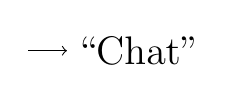
\begin{tikzpicture}
  \usetikzlibrary{calc}
  \usetikzlibrary{3d}

  \def\scale{4}
  \def\alexx{0}
  \def\alexy{0}
  \def\alexz{0}

  \def\coblue{blue!50!gray}
  \def\coorange{orange!50!gray}
  \def\cogreen{green!50!gray}
  \def\copurple{purple!50!white}

  \imagelayer{1.3*\scale}{-0.8*\scale+\alexx}{\alexy}{\alexz}{nobu}{Image}{3}
  \convlayer{1.3*\scale}{1.3*\scale}{0.02*\scale}{Image}{\coblue}{-0.05*\scale+\alexx}{\alexy}{\alexz}{{224}{224}{3}}
  \convlayer{1.1*\scale}{1.1*\scale}{0.1*\scale}{Conv1}{\coblue}{\alexx+0.6*\scale}{\alexy}{\alexz}{{55}{55}{96}}
  \convlayer{0.7*\scale}{0.7*\scale}{0.1*\scale}{Pool1}{\coorange}{\alexx+1*\scale}{\alexy}{\alexz}{{}{}{96}}
  \convlayer{0.7*\scale}{0.7*\scale}{0.1*\scale}{LRN}{\cogreen}{\alexx+1.35*\scale}{\alexy}{\alexz}{{}{}{96}}
  \convlayer{0.7*\scale}{0.7*\scale}{0.4*\scale}{Conv2}{\coblue}{\alexx+2*\scale}{\alexy}{\alexz}{{27}{27}{256}}
  \convlayer{0.5*\scale}{0.5*\scale}{0.1*\scale}{Pool2}{\coorange}{\alexx+2.5*\scale}{\alexy}{\alexz}{{}{}{}}
  \convlayer{0.5*\scale}{0.5*\scale}{0.1*\scale}{LRN}{\cogreen}{\alexx+2.75*\scale}{\alexy}{\alexz}{{}{}{}}
  \convlayer{0.5*\scale}{0.5*\scale}{0.6*\scale}{Conv3}{\coblue}{\alexx+3.35*\scale}{\alexy}{\alexz}{{}{}{384}}
  \convlayer{0.5*\scale}{0.5*\scale}{0.6*\scale}{Conv4}{\coblue}{\alexx+4.2*\scale}{\alexy}{\alexz}{{}{}{384}}
  \convlayer{0.5*\scale}{0.5*\scale}{0.4*\scale}{Conv5}{\coblue}{\alexx+5*\scale}{\alexy}{\alexz}{{}{}{256}}
  \convlayer{0.3*\scale}{0.3*\scale}{0.1*\scale}{Pool5}{\coorange}{\alexx+5.5*\scale}{\alexy}{\alexz}{{}{}{256}}
  \fclayer{\scale}{0.1*\scale}{FC1}{\copurple}{\alexx+5.8*\scale}{\alexy}{\alexz}{4096}
  \fclayer{\scale}{0.1*\scale}{FC2}{\copurple}{\alexx+6.05*\scale}{\alexy}{\alexz}{4096}
  \fclayer{\scale}{0.1*\scale}{FC3}{\copurple}{\alexx+6.3*\scale}{\alexy}{\alexz}{1000}
  \node (out) at (\alexx+6.7*\scale,\alexy) {\Large ``Chat''};
  \draw[->] (\alexx+6.35*\scale,\alexy) -- (out.west);

  \end{tikzpicture}
\end{document}

  }
  \caption{Architecture AlexNet~\cite{krizhevsky_imagenet_2012}}
  \label{fig:alexnet}
\end{figure}

\begin{figure}
  \resizebox{\textwidth}{!}{
    \documentclass{standalone}
\usepackage[utf8]{inputenc}
\usepackage[T1]{fontenc}
\usepackage{tikz}
\usepackage{ifthen}
\input{../CommandesPerso.tex}

\begin{document}
  \begin{tikzpicture}
  \usetikzlibrary{calc}
  \usetikzlibrary{3d}

  \def\scale{3.5}
  \def\vggx{0}
  \def\vggy{0}
  \def\vggz{0}

  \def\coblue{blue!50!gray}
  \def\coorange{orange!70!gray}
  \def\cogreen{green!50!gray}
  \def\copurple{purple!50!white}

  \imagelayer{1.3*\scale}{0.1*\scale+\vggx}{\vggy}{\vggz}{nobu}{Image}{$224\times224\times3$}
  \convlayer{1.1*\scale}{1.1*\scale}{0.04*\scale}{Conv1-2}{\coblue}{\vggx+0.6*\scale}{\vggy}{\vggz}{{}{}{64}}
  \convlayer{1.1*\scale}{1.1*\scale}{0.04*\scale}{}{\coblue}{\vggx+0.7*\scale}{\vggy}{\vggz}{{}{}{64}}
  \convlayer{0.8*\scale}{0.8*\scale}{0.04*\scale}{Pool1}{\coorange}{\vggx+1*\scale}{\vggy}{\vggz}{{112}{112}{}}
  \convlayer{0.8*\scale}{0.8*\scale}{0.08*\scale}{Conv3-4}{\coblue}{\vggx+1.2*\scale}{\vggy}{\vggz}{{}{}{128}}
  \convlayer{0.8*\scale}{0.8*\scale}{0.08*\scale}{}{\coblue}{\vggx+1.35*\scale}{\vggy}{\vggz}{{112}{}{128}}
  \convlayer{0.6*\scale}{0.6*\scale}{0.08*\scale}{Pool2}{\coorange}{\vggx+1.7*\scale}{\vggy}{\vggz}{{}{56}{}}
  \convlayer{0.6*\scale}{0.6*\scale}{0.2*\scale}{Conv5-7}{\coblue}{\vggx+2*\scale}{\vggy}{\vggz}{{}{}{256}}
  \convlayer{0.6*\scale}{0.6*\scale}{0.2*\scale}{}{\coblue}{\vggx+2.25*\scale}{\vggy}{\vggz}{{}{}{256}}
  \convlayer{0.6*\scale}{0.6*\scale}{0.2*\scale}{}{\coblue}{\vggx+2.5*\scale}{\vggy}{\vggz}{{56}{}{256}}
  \convlayer{0.3*\scale}{0.3*\scale}{0.2*\scale}{Pool3}{\coorange}{\vggx+2.9*\scale}{\vggy}{\vggz}{{28}{28}{}}
  \convlayer{0.3*\scale}{0.3*\scale}{0.4*\scale}{Conv8-10}{\coblue}{\vggx+3.4*\scale}{\vggy}{\vggz}{{}{}{512}}
  \convlayer{0.3*\scale}{0.3*\scale}{0.4*\scale}{}{\coblue}{\vggx+3.9*\scale}{\vggy}{\vggz}{{}{}{512}}
  \convlayer{0.3*\scale}{0.3*\scale}{0.4*\scale}{}{\coblue}{\vggx+4.4*\scale}{\vggy}{\vggz}{{14}{}{512}}
  \convlayer{0.3*\scale}{0.3*\scale}{0.2*\scale}{Pool4}{\coorange}{\vggx+4.95*\scale}{\vggy}{\vggz}{{14}{14}{}}
  \convlayer{0.3*\scale}{0.3*\scale}{0.4*\scale}{Conv11-13}{\coblue}{\vggx+5.45*\scale}{\vggy}{\vggz}{{}{}{512}}
  \convlayer{0.3*\scale}{0.3*\scale}{0.4*\scale}{}{\coblue}{\vggx+5.95*\scale}{\vggy}{\vggz}{{}{}{512}}
  \convlayer{0.3*\scale}{0.3*\scale}{0.4*\scale}{}{\coblue}{\vggx+6.45*\scale}{\vggy}{\vggz}{{14}{}{512}}
  \convlayer{0.15*\scale}{0.15*\scale}{0.4*\scale}{Pool5}{\coorange}{\vggx+7.05*\scale}{\vggy}{\vggz}{{7}{7}{512}}

  \fclayer{\scale}{0.1*\scale}{FC1}{\copurple}{\vggx+7.4*\scale}{\vggy}{\vggz}{4096}
  \fclayer{\scale}{0.1*\scale}{FC2}{\copurple}{\vggx+7.6*\scale}{\vggy}{\vggz}{4096}
  \fclayer{0.8*\scale}{0.1*\scale}{FC3}{\copurple}{\vggx+7.8*\scale}{\vggy}{\vggz}{1000}
  \node (out) at (\vggx+8.2*\scale,\vggy) {\Large ``Chat''};
  \draw[->] (\vggx+7.85*\scale,\vggy) -- (out.west);

  \end{tikzpicture}
\end{document}

  }
  \caption{Architecture VGG-16~\cite{simonyan_very_2014}}
  \label{fig:vgg}
\end{figure}

\begin{figure}
  \resizebox{\textwidth}{!}{
    \documentclass{standalone}
\usepackage[utf8]{inputenc}
\usepackage[T1]{fontenc}
\usepackage{tikz}
\usepackage{ifthen}
\usepackage{graphicx}
\input{../CommandesPerso.tex}

\begin{document}
  \begin{tikzpicture}
  \usetikzlibrary{calc}
  \usetikzlibrary{3d}

  \def\scale{4}
  \def\vggx{0}
  \def\vggy{0}
  \def\vggz{0}

  \def\coblue{blue!50!gray}
  \def\cored{red!50!gray}
  \def\coorange{orange!70!gray}
  \def\cogreen{green!50!gray}
  \def\copurple{purple!50!white}

  \imagelayer{1.3*\scale}{-0.3*\scale+\vggx}{\vggy}{\vggz}{nobu}{Image}{$224\times224\times3$}
  \convlayer{1.3*\scale}{1.3*\scale}{0.02*\scale}{Image}{\coblue}{0.2*\scale+\vggx}{\vggy}{\vggz}{{224}{}{3}}
  \convlayer{1*\scale}{1*\scale}{0.04*\scale}{Conv1}{\coblue}{\vggx+0.6*\scale}{\vggy}{\vggz}{{112}{112}{64}}
  \convlayer{0.8*\scale}{0.8*\scale}{0.04*\scale}{Pool1}{\coorange}{\vggx+1*\scale}{\vggy}{\vggz}{{56}{56}{}}
  \convlayer{0.8*\scale}{0.8*\scale}{0.15*\scale}{Conv2}{\coblue}{\vggx+1.4*\scale}{\vggy}{\vggz}{{}{}{192}}
  \convlayer{0.6*\scale}{0.6*\scale}{0.15*\scale}{Pool2}{\coorange}{\vggx+1.8*\scale}{\vggy}{\vggz}{{28}{28}{}}
  \node at (\vggx+2.45*\scale, \vggy+0.5*\scale) {Inception (3a-3b)};
  \convlayer{0.6*\scale}{0.6*\scale}{0.2*\scale}{}{\cored}{\vggx+2.2*\scale}{\vggy}{\vggz}{{}{}{256}}
  \convlayer{0.6*\scale}{0.6*\scale}{0.3*\scale}{}{\cored}{\vggx+2.5*\scale}{\vggy}{\vggz}{{}{}{480}}
  \convlayer{0.4*\scale}{0.4*\scale}{0.3*\scale}{Pool3}{\coorange}{\vggx+2.9*\scale}{\vggy}{\vggz}{{14}{14}{}}
  \node at (\vggx+4.5*\scale, \vggy+0.4*\scale) {Inception (4a-4e)};
  \convlayer{0.4*\scale}{0.4*\scale}{0.4*\scale}{}{\cored}{\vggx+3.4*\scale}{\vggy}{\vggz}{{}{}{512}}
  \convlayer{0.4*\scale}{0.4*\scale}{0.4*\scale}{}{\cored}{\vggx+3.9*\scale}{\vggy}{\vggz}{{}{}{512}}
  \convlayer{0.4*\scale}{0.4*\scale}{0.4*\scale}{}{\cored}{\vggx+4.4*\scale}{\vggy}{\vggz}{{}{}{512}}
  \convlayer{0.4*\scale}{0.4*\scale}{0.4*\scale}{}{\cored}{\vggx+4.9*\scale}{\vggy}{\vggz}{{}{}{528}}
  \convlayer{0.4*\scale}{0.4*\scale}{0.5*\scale}{}{\cored}{\vggx+5.4*\scale}{\vggy}{\vggz}{{}{}{832}}
  \convlayer{0.3*\scale}{0.3*\scale}{0.5*\scale}{Pool5}{\coorange}{\vggx+6.1*\scale}{\vggy}{\vggz}{{}{}{832}}
  \node at (\vggx+7*\scale, \vggy+0.4*\scale) {Inception (5a-5b)};
  \convlayer{0.3*\scale}{0.3*\scale}{0.5*\scale}{}{\cored}{\vggx+6.7*\scale}{\vggy}{\vggz}{{}{}{832}}
  \convlayer{0.3*\scale}{0.3*\scale}{0.6*\scale}{}{\cored}{\vggx+7.3*\scale}{\vggy}{\vggz}{{}{}{1024}}
  \node at (\vggx+8.05*\scale, \vggy+0.2*\scale) {Avg. pool};
  \convlayer{0.1*\scale}{0.1*\scale}{0.6*\scale}{}{\coorange}{\vggx+8.05*\scale}{\vggy}{\vggz}{{}{}{$1\times1\times1024$}}
  \fclayer{\scale}{0.1*\scale}{FC}{\copurple}{\vggx+8.5*\scale}{\vggy}{\vggz}{1000}
  \node (out) at (\vggx+8.9*\scale,\vggy) {\Large ``Chat''};
  \draw[->] (\vggx+8.55*\scale,\vggy) -- (out.west);

  \end{tikzpicture}
\end{document}

  }
  \caption{Architecture GoogLeNet~\cite{szegedy_going_2015}}
  \label{fig:googlenet}
\end{figure}

\missingfigure{inception module}

\begin{figure}
  \resizebox{\textwidth}{!}{
    \documentclass{standalone}
\usepackage[utf8]{inputenc}
\usepackage[T1]{fontenc}
\usepackage{tikz}
\usepackage{ifthen}
\usepackage{graphicx}
\input{../CommandesPerso.tex}

\begin{document}
  \begin{tikzpicture}
  \usetikzlibrary{calc}
  \usetikzlibrary{3d}

  \def\scale{4}
  \def\vggx{0}
  \def\vggy{0}
  \def\vggz{0}

  \def\coblue{blue!50!gray}
  \def\cored{red!50!gray}
  \def\coorange{orange!70!gray}
  \def\cogreen{green!50!gray}
  \def\copurple{purple!50!white}

  \imagelayer{1.3*\scale}{-0.3*\scale+\vggx}{\vggy}{\vggz}{nobu}{Image}{$224\times224\times3$}
  \convlayer{1.3*\scale}{1.3*\scale}{0.02*\scale}{Image}{\coblue}{0.2*\scale+\vggx}{\vggy}{\vggz}{{224}{}{3}}
  \convlayer{1*\scale}{1*\scale}{0.04*\scale}{Conv1}{\coblue}{\vggx+0.6*\scale}{\vggy}{\vggz}{{112}{112}{64}}
  \convlayer{0.8*\scale}{0.8*\scale}{0.04*\scale}{Pool1}{\coorange}{\vggx+1*\scale}{\vggy}{\vggz}{{56}{56}{}}

  \foreach \ratio [count=\ni] in {1.4,1.5,1.6,1.7,1.8,1.9}{
  \convlayer{0.8*\scale}{0.8*\scale}{0.04*\scale}{}{\coblue}{\vggx+\ratio*\scale}{\vggy}{\vggz}{{}{}{64}}
  \ifnum\ni=1%
      \draw (\vggx+\ratio*\scale-0.3*\scale, \vggy+0.5*\scale) edge[dashed,thick,->,in=90,out=90,looseness=2] (\vggx+\ratio*\scale, \vggy+0.4*\scale);
  \else%
      \draw (\vggx+\ratio*\scale-0.1*\scale+0.035*\scale, \vggy+0.4*\scale) edge[thick,->,in=90,out=90,looseness=10] (\vggx+\ratio*\scale, \vggy+0.4*\scale);
  \fi%
  }


  \foreach \ratio [count=\ni] in {2.2,2.35,2.5,2.65,2.8,2.95,3.10,3.25}{
  \convlayer{0.6*\scale}{0.6*\scale}{0.08*\scale}{}{\coblue}{\vggx+\ratio*\scale}{\vggy}{\vggz}{{}{}{128}}
  \ifnum\ni=1%
      \draw (\vggx+\ratio*\scale-0.2*\scale, \vggy+0.5*\scale) edge[dashed,looseness=2,thick,->,in=90,out=90] (\vggx+\ratio*\scale, \vggy+0.3*\scale);%
  \else%
      \draw (\vggx+\ratio*\scale-0.15*\scale+0.035*\scale, \vggy+0.3*\scale) edge[looseness=5,thick,->,in=90,out=90] (\vggx+\ratio*\scale, \vggy+0.3*\scale);%
  \fi%
  }

  \foreach \ratio [count=\ni] in {3.5,3.7,3.9,4.1,4.3,4.5,4.7,4.9,5.1,5.3,5.5,5.7}{
  \convlayer{0.4*\scale}{0.4*\scale}{0.12*\scale}{}{\coblue}{\vggx+\ratio*\scale}{\vggy}{\vggz}{{}{}{256}}
  \ifnum\ni=1%
      \draw (\vggx+\ratio*\scale-0.2*\scale, \vggy+0.3*\scale) edge[dashed,thick,looseness=1.5,->,in=90,out=90] (\vggx+\ratio*\scale, \vggy+0.2*\scale);
  \else%
      \draw (\vggx+\ratio*\scale-0.2*\scale+0.035*\scale, \vggy+0.2*\scale) edge[thick,looseness=2,->,in=90,out=90] (\vggx+\ratio*\scale, \vggy+0.2*\scale);
  \fi%
  }

  \foreach \ratio [count=\ni] in {6,6.3,6.6,6.9,7.2,7.5,7.8}{
  \convlayer{0.3*\scale}{0.3*\scale}{0.2*\scale}{}{\coblue}{\vggx+\ratio*\scale}{\vggy}{\vggz}{{}{}{512}}
  \ifnum\ni=1%
      \draw (\vggx+\ratio*\scale-0.3*\scale+0.05*\scale, \vggy+0.225*\scale) edge[dashed,thick,->,in=90,out=90,looseness=1.25] (\vggx+\ratio*\scale, \vggy+0.15*\scale);
  \else%
      \draw (\vggx+\ratio*\scale-0.3*\scale+0.05*\scale, \vggy+0.15*\scale) edge[thick,->,in=90,out=90,looseness=1.5] (\vggx+\ratio*\scale, \vggy+0.15*\scale);
  \fi%
  }

  \node at (\vggx+8.3*\scale, \vggy+0.2*\scale) {Avg. pool};
  \convlayer{0.1*\scale}{0.1*\scale}{0.6*\scale}{}{\coorange}{\vggx+8.3*\scale}{\vggy}{\vggz}{{}{}{$1\times1\times1024$}}
  \fclayer{\scale}{0.1*\scale}{FC}{\copurple}{\vggx+8.7*\scale}{\vggy}{\vggz}{1000}
  \node (out) at (\vggx+9.1*\scale,\vggy) {\Large ``Chat''};
  \draw[->] (\vggx+8.75*\scale,\vggy) -- (out.west);

  \end{tikzpicture}
\end{document}

  }
  \caption{Architecture ResNet-34~\cite{he_deep_2016}}
  \label{fig:googlenet}
\end{figure}

\missingfigure{residual connection}

\missingfigure{densenet}

Des progrès considérables ont été réalisés depuis le succès d'AlexNet~\cite{krizhevsky_imagenet_2012}, notamment\,:
les modèles VGG~\cite{chatfield_return_2014} et \cite{simonyan_very_2014}
le modèle Inception~\cite{szegedy_going_2015} et ses variantes~\cite{szegedy_rethinking_2015,szegedy_inception-v4_2016}
Le modèle ResNet~\cite{he_deep_2016}
Puis le modèle DenseNet~\cite{huang_densely_2017}

Toutefois, la classification d'images ne donne aucune information particulière de localisation, seulement une information binaire de présence d'un objet dans une image. Des approches à base de réseaux profonds pour la détection d'objet à partir de classification de sous-régions de l'image ont rapidement vu le jour~\cite{girshick_rich_2014,liu_ssd_2016,girshick_region-based_2016} supplantant les approches traditionnelles de localisation~\cite{lowe_object_1999,dalal_histograms_2005,gu_recognition_2009,uijlings_selective_2013}. Cependant, ces approches ne répondent pas exactement au problème décrit par Papert en 1966. La question n'est pas uniquement de pouvoir identifier des objets, mais aussi d'en estimer la forme et de les séparer du fond. Cette tâche consiste donc à la segmentation sémantique, c'est-à-dire à l'association d'une classe d'intérêt non pas à chaque image, mais à chaque pixel.

Plusieurs jeux de données ont été introduits dans la communauté vision par ordinateur afin d'évaluer des méthodes sur cette tâche, notamment sur des scènes de la vie quotidienne, comme PASCAL VOC~\cite{everingham_pascal_2014}, Microsoft COCO~\cite{lin_microsoft_2014} et également sur des scènes de conduite autonome avec des jeux de données tels que CamVid~\cite{brostow_semantic_2009}, Cityscapes~\cite{cordts_cityscapes_2016} ou encore Mapillary Vistas~\cite{neuhold_mapillary_2017}. Les premières approches de segmentation sémantique ont réalisé des classification à partir de caractéristiques denses calculées sur l'ensemble de l'image, regroupées \emph{a posterio} par régions homogènes~\cite{shotton_semantic_2008,shotton_real-time_2011}. Les réseaux convolutifs profonds également utilisés à cette fin en calculant une classification pour chaque pixel de l'image~\cite{grangier_deep_2009,ciresan_deep_2012} ou pour chaque région~\cite{farabet_towards_2013,sermanet_overfeat_2013}. Une observation importante est que les cartes de caractéristiques issues des couches convolutives conservent la structure spatiale de l'image, c'est-à-dire qu'il est possible de faire correspondre chaque caractéristique à un ou plusieurs pixels. Cette extraction de caractéristique dense se prête particulièrement aux problématiques de localisation d'objet et est rapidement adoptée par la communauté~\cite{zou_generic_2014}.

\subsection{Approches entièrement convolutives}

\missingfigure{Convolutionalisation}

La forme moderne des réseaux convolutifs profonds pour la segmentation sémantique est popularisée par~\citet{long_fully_2015}. L'idée fondamentale est de ne manipuler que des réseaux entièrement convolutifs, c'est-à-dire sans couche entièrement connectées. Dès lors, les cartes d'activation conservent leurs propriétés spatiales et peuvent être relocalisées sur l'image originale par un simple jeu de sur-échantillonnage, par exemple par interpolation bilinéaire. L'approche choisie par~\citet{long_fully_2015} leur permet de produire des prédictions denses à résolution 1:32, 1:16 et 1:8. Cette approche permettent immédiatement d'établir de nouveaux état de l'art sur les jeux de données de segmentation sémantique et dominent largement les compétitions depuis 2015.

Cette approche est reprise et améliorée selon plusieurs axes. Tout d'abord, en gardant la structure des couches convolutives de VGG-16~\cite{simonyan_very_2014},~\citet{l._c._chen_deeplab_2018} proposent d'une part d'utiliser les convolutions à trous pour agrandir le champ réceptif du réseau et retirer les couches de \emph{maxpooling} qui réduisent la résolution spatiale, et d'autre part d'utiliser un \gls{CRF} \emph{a posteriori} pour régulariser les cartes prédites. De façon similaire,~\citet{yu_multi-scale_2015} proposent l'utilisation de la convolution à trous (nommée convolution dilatée) pour agréger des cartes d'activation à plusieurs échelles. Les \gls{CRF} sont également manipulés de manière à s'exprimer sous forme d'un réseau récurrent optimisable conjointement avec le \gls{FCN}~\cite{zheng_conditional_2015} ou comme rafinement~\cite{arnab_higher_2015}.

Une approche dérivée des auto-encodeurs convolutifs~\cite{zhao_stacked_2015-1} est proposée, en utilisant soit la déconvolution pour recomposer la résolution spatiale~\cite{ronneberger_u-net_2015,nekrasov_global_2016,noh_learning_2015}, soit le sur-échantillonnage~\cite{badrinarayanan_segnet_2017}.

Le passage aux architectures ResNet~\cite{wu_high-performance_2016} puis DenseNet~\cite{jegou_one_2017} permettent d'améliorer encore les performances mais au prix d'un surcoût calculatoire conséquent.

\todo[inline]{large kernel matters (papier), gridnet (papier)}
Diverses approches multi-échelles sont proposées, aussi bien dans DeepLab~\cite{l._c._chen_deeplab_2018} en utilisant des prédictions à plusieurs résolutions que par des approches utilisant des noyaux de convolution à différentes tailles, soit via la dilation~\cite{yu_multi-scale_2015}, soit par des convolutions parallèle à la Inception~\cite{szegedy_going_2015,nekrasov_global_2016,zhao_pyramid_2017}.

\section{Apprentissage pour le traitement d'images de télédétection}

\subsection{Différents types d'imagerie}

La télédétection et en particulier l'observation de la Terre comprend une grande variété de capteurs d'imageries. Contrairement au multimédia, ces capteurs peuvent être de nature très variables. Si les acquisitions aéroportées se font généralement en couleurs \gls{RVB} à l'aide d'appareils photos clasiques, les acquisitions satellitaires utilisent bien souvent des capteurs dotés de capacités particulière, comme de remonter une information spectrale riche, percer la couverture nuageuse ou mesurer des propriétés physiques de la surface de la Terre.

Le cas plus simple à envisager est celui de l'infrarouge. Il est courant, y compris dans les acquisitions d'images aéroportées, d'imager aussi bien le domaine visible que le proche infrarouge, situé entre \SI{780}{\nano\meter} et \SI{2 500}{\nano\meter}, notamment car la végétation y a une réponse amplifiée par la présence de chlorophylle. Dans l'infrarouge moyen et lointain, il est également possible de mesurer indirectement la température grâce aux radiations lumineuses émises grâce à la loi de Wien. Ces caméras thermiques sont particulièrement utiles dans l'espace, car cela permet de s'affranchir du bruit ambiant causé par la chaleur naturelle terrestre.

\begin{figure}
  \resizebox{\textwidth}{!}{
  \documentclass{standalone}
\usepackage[utf8]{inputenc}
\usepackage[T1]{fontenc}
\usepackage{tikz}
\usepackage{pgfplots}
\input{../CommandesPerso}
\begin{document}

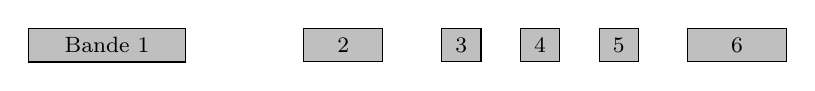
\begin{tikzpicture}
\lightspectrum

\node[draw,fill=gray!50!white,minimum width=2cm,rectangle] at (3.5, -0.2) {\footnotesize Bande 1};
\node[draw,fill=gray!50!white,minimum width=1cm,rectangle] at (6.5, -0.2) {\footnotesize 2};
\node[draw,fill=gray!50!white,minimum width=0.5cm,rectangle] at (8, -0.2) {\footnotesize 3};
\node[draw,fill=gray!50!white,minimum width=0.5cm,rectangle] at (9, -0.2) {\footnotesize 4};
\node[draw,fill=gray!50!white,minimum width=0.5cm,rectangle] at (10, -0.2) {\footnotesize 5};
\node[draw,fill=gray!50!white,minimum width=1.25cm,rectangle] at (11.5, -0.2) {\footnotesize 6};
\end{tikzpicture}
\end{document}

  }
  \caption{Exemple de répartitions de bandes spectrales dans les domaines spectraux lumineux.}
  \label{fig:multispectral}
\end{figure}

En étendant ce principe, une caméra multispectrale ou superspectrale va imager une scène non pas seulement dans les trois canaux habituels \gls{RVB} dans le domaine visible, mais dans plusieurs bandes de longueurs d'ondes plus ou moins larges pouvant se trouver aussi bien dans le visible que dans l'infrarouge ou l'ultraviolet, comme illustré dans la~\cref{fig:multispectral}. Cela conduit à des images à plusieurs canaux, généralement aux alentours d'une dizaine, qui ne sont donc pas directement visualisables par l'\oe{}il humain. Il est toutefois possible de reconstituer une image en couleurs naturelles en recomposant une image \gls{RVB} à partir des valeurs contenues dans les canaux correspondant aux longueurs d'onde du rouge, du vert et du bleu. Les acquistions multispectrales peuvent avoir des résolutions différentes en fonction des canaux. Les satellites Sentinel-2A et Sentinel-2B produisent par exemple des images à une résolution au sol de \SI{10}{\meter/\px} dans le domaine visible, mais certaines bandes, notamment dans l'infrarouge, ont des résolutions de \SI{20}{\meter/\px} ou \SI{60}{\meter/\px}. Les acquisitions couleurs satellitaires les mieux résolues spatialement ont une résolution au sol de l'ordre de \SI{50}{\centi\meter/\px}, tandis que les images aéroportées peuvent aller jusqu'à une résolution de \SI{5}{\centi\meter/\px}. Dans le cas des acquisitions satellitaires, il est courant de réaliser en simultanée une mesure multispectrale et une acquisition panchromatique, c'est-à-dire qui ne distingue pas les couleurs et produit une image en noir et blanc, à résolution supérieure. Ainsi, \gls{Pleiades} réalise à la fois une acquisition panchromatique à résolution \SI{70}{\centi\meter/\px}, rééchantillonnée à \SI{50}{\centi\meter/\px} et multispectrale à \SI{2,8}{\meter} rééchantilonnée à \SI{2}{\meter}.

\begin{figure}
  \resizebox{\textwidth}{!}{
  \documentclass{standalone}
\usepackage[utf8]{inputenc}
\usepackage[T1]{fontenc}
\usepackage{tikz}
\usepackage{pgfplots}
\input{../CommandesPerso}
\begin{document}

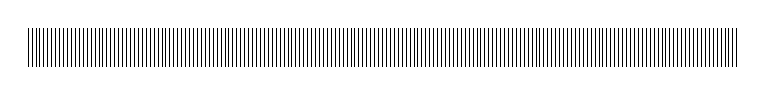
\begin{tikzpicture}
\lightspectrum

\foreach \x in {300,305,...,1200}{
\fill (\x/100, -0.5) rectangle (\x/100+0.01, 0.);
}
\end{tikzpicture}
\end{document}

  }
  \caption{Exemple de répartitions de bandes spectrales dans les domaines spectraux lumineux.}
  \label{fig:hyperspectral}
\end{figure}

L'imagerie hyperspectrale consiste à effectuer des acquisitions sur de nombreuses bandes étroites, toutes de même taille, afin de balayer de façon discrète l'ensemble du spectre lumineux réfléchi, comme illustré par la~\cref{fig:hyperspectral}. En fonction de la résolution spectrale -- souvent de l'ordre de \SI{10}{\nano\meter} -- et de la largeur du spectre considéré, le nombre de bandes peut varier de quelques dizaines à plusieurs centaines. L'avantage principale de ce type de caméra est qu'il est possible pour un pixel donné de reconstituer la courbe de l'intensité lumineuse réfléchie en fonction de la longueur d'onde. Chaque matériau réfléchit différemment la lumière en fonction de son albédo et cette information permet donc de caractériser finement la composition des objets d'intérêt observés. Toutefois, les caméras hyperspectrales ont également une résolution spatiale nettement plus faibles que les caméras \gls{RVB} ou multispectrales classiques, produisant des images à une résolution au sol d'environ \SI{1}{\meter/\px} en aérien.

Il est important de noter que ces capteurs optiques sont passifs. Ils ne reçoivent que l'énergie lumineuse réfléchie ou émise par le corps observé, ce qui restreint ce qu'il est possible de réaliser. Notamment, ces capteurs sont sensibles aux variations d'illumination et aux effets météorologiques, en particulier la couche nuageuse qui les rendre entièrement inopérationnels. Ainsi, de nombreux satellites sont eux munis de capteurs actifs qui émettent un signal et mesurent le retour de celui-ci. C'est cette approche qui est utilisée pour les satellites radar, et notamment \gls{SAR}, qui envoient une ou plusieurs ondes électromagnétiques et utilisent la mesure de l'onde réfléchie pour extraire des paramètres physiques de la zone observée.

\begin{figure}
  \resizebox{\textwidth}{!}{
  \input{Chapitre1/mnt.pdf_tex}
  }
  \caption{Schéma représentatif de la différence entre \gls{MNT} et \gls{MNE}.}
  \label{fig:mnt}
\end{figure}

En outre, le \gls{Lidar} est un capteur actif émettant une impulsion laser dont il mesure l'écho. La position du maximum d'amplitude permet de déterminer le temps d'aller-retour du signal lumineux et donc de mesurer la distance parcourue par les photons. Ces capteurs sont très utilisés aussi bien en télédétection qu'en robotique pour effectuer des relevés topographiques et la reconstruction 3D. L'inconvénient principal du \gls{Lidar} est que la mesure laser est ponctuelle et qu'il ne permet donc que de construire des nuages de points peu denses. Dans le cas du \gls{Lidar} satellitaire, les points de mesure sont généralement espacés d'environ \SI{20}{\meter}, et \SI{10}{\centi\meter} dans le cas de l'aéroporté. Une fois le nuage de points construit, il est possible d'en extraire un maillage qui modélise la topographie de la surface observée. Il est ensuite possible de rastériser ce maillage pour obtenir un \gls{MNT} ou un \gls{MNE} en fonction de la résolution. Le \gls{MNE} se distingue du \gls{MNT} en ce qu'il prend en compte les objets surélevés par-dessus la surface topographique, comme illustré par la~\cref{fig:mnt}. La différence entre ces deux modèles est appelée \gls{MNH} et correspond à la hauteur normalisée des points au-dessus du sol.

Nos travaux portent principalement sur l'utilisation de données optiques pour la cartographie automatisée, cependant, nous utiliserons également des données issues de capteurs \gls{Lidar}.

\subsection{Jeux de données en télédétection}

Il existe plusieurs jeux de données pour la classification d'images optiques de télédétection. Citons ainsi les jeux de données UC Merced~\cite{yang_bag--visual-words_2010} contenant 2 100 images aériennes dans 21 classes d'occupation des sols, Brazilian Coffe~\cite{penatti_deep_2015} d'images \gls{SPOT} pour la classification de terrains cultivés et SAT-4/SAT-6~\cite{basu_deepsat_2015} contenant respectivement 500 000 et 405 000 images aériennes pour plusieurs classes d'occupation des sols. L'inconvénient de ces jeux de données est d'une part la faible taille des images (256$\times$\SI{256}{\px} pour UC Merced et Brazilian Coffe, $28\times28$\SI{}{\px} pour SAT) et la faible quantité d'annotations. En effet, ces jeux de données, prévus pour la classification, ne peuvent que difficilement être utilisés pour la segmentation sémantique.

Cependant, plusieurs jeux de données comprenant des annotations denses ont été proposés.

\subsubsection{ISPRS 2D Semantic Labeling}

\begin{figure}[t]
	\begin{subfigure}{0.5\textwidth}
		\foreach\picid in {7,21,28}{%
		\begin{subfigure}{0.33\textwidth}
			\includegraphics[width=\textwidth]{vaihingen_top_\picid}
			\caption*{Image RVB}
		\end{subfigure}%
		\begin{subfigure}{0.33\textwidth}
			\includegraphics[width=\textwidth]{vaihingen_ndsm_\picid}
			\caption*{\gls{MNH}}
		\end{subfigure}%
		\begin{subfigure}{0.33\textwidth}
			\includegraphics[width=\textwidth]{vaihingen_top_\picid}
			\caption*{Vérité terrain}
		\end{subfigure}
		}
	\end{subfigure}%
	\begin{subfigure}{0.5\textwidth}
		\foreach\picid in {3_10,6_11,7_12}{%
		\begin{subfigure}{0.33\textwidth}
			\includegraphics[width=\textwidth]{potsdam_top_\picid}
			\caption*{Image RVB}
		\end{subfigure}%
		\begin{subfigure}{0.33\textwidth}
			\includegraphics[width=\textwidth]{potsdam_ndsm_\picid}
			\caption*{\gls{MNH}}
		\end{subfigure}%
		\begin{subfigure}{0.33\textwidth}
			\includegraphics[width=\textwidth]{potsdam_gt_\picid}
			\caption*{Vérité terrain}
		\end{subfigure}
		}
	\end{subfigure}
	\caption{Images ortho-rectifiées et \gls{MNH} pour les jeux de données ISPRS Vaihingen et ISPRS Potsdam.}
	\label{fig:isprs_dataset}
\end{figure}

Le jeu de données ISPRS 2D Semantic Labeling~\cite{rottensteiner_isprs_2012} est constitué de deux ensembles d'images aériennes \glsfirst{THR}. Dans les deux cas, il s'agit de scènes urbaines diposant de cinq classes d'intérêt pour la segmentation sémantique\,: surfaces imperméables (routes, parkings, trottoirs\dots), bâtiments, végétation basse, arbres et véhicules. Une classe de rejet est également définie et comprend le mobilier urbain (bancs, poubelles, conteneurs\dots) et les surfaces exotiques (terrains de basketball, zones en travaux, points d'eau).

Le jeu de données se décline en deux scènes. La première est issue d'une acquisition aéroportée sur la ville de Vaihingen (Allemagne) et comporte une mosaïque de 33 tuiles \gls{IRRV} ortho-rectifiées à une résolution de 9cm/px. L'acquisition optique est accompagnée d'une acquisition \gls{Lidar} à la même résolution, dont a été extrait un \gls{MNE}. Un \gls{MNH} pré-calculé~\cite{gerke_use_2015} dérivé du \gls{MNE} est également disponible. Les ortho-images sont fournies en format \gls{TIFF} encodés sur 8 bits, tandis que le \gls{MNE} est fourni en flottant sur 32 bits. Toutes les données ont été recalées sur la même grille de pixels. Les images ont une taille moyenne d'environ $2600\times1900$px, soit une surface d'approximativement $40 000m^2$. Vaihingen est une ville de taille moyenne (28 853 habitants en 2009), caractérisée par une urbanisation moyenne composée majoritairement de pavillons résidentiels et d'espace verts urbains.

La seconde scène est une acquisition aéroportée sur la ville de Potsdam (Allemagne) et comporte une mosaïque de 38 tuiles \gls{IRRVB} à une résolution de 5cm/px. Les tuiles présentent toutes les mêmes dimensions, à savoir $6000\times6000$px, soit une surface de $90 000m^2$. Un \gls{MNE} et un \gls{MNH} dérivé sont également fournis. Des annotations denses sont disponibles pour les mêmes classes que précédemment sur 24 images. À nouveau, l'ensemble des modalités sont recalées sur la même grille de pixels et les images sont fournies en \gls{TIFF} sur 8 bits, tandis que les modèles de surface sont fournis en flottant sur 32 bits. Potsdam est une ville urbanisée relativement grande (161 468 habitants en 2013), caractérisée par de nombreux immeubles, un réseau routier dense. À noter la présence d'un canal et de nombreux travaux de construction à la date de l'acquisition des images.

Quelques exemples représentatifs des deux acquisitions sont montrés dans la~\cref{fig:isprs_dataset}.

Les images dont les annotations ne sont pas rendues publiques servent à évaluer en aveugle les méthodes proposées par la communauté. La commission WG II/4 de l'\gls{ISPRS} gère ainsi un tableau de résultat public\footnote{\url{http://www2.isprs.org/commissions/comm2/wg4/vaihingen-2d-semantic-labeling-contest.html}}\footnote{\url{http://www2.isprs.org/commissions/comm2/wg4/potsdam-2d-semantic-labeling.html}}, détaillant les performances obtenues par différentes méthodes de l'état-de-l'art.

\subsubsection{Data Fusion Contest 2015}

Le jeu de données \gls{DFC} 2015~\cite{campos-taberner_processing_2016} est issu d'une compétition de fusion de données organisée par le groupe de travail \gls{GRSS} de l'\gls{IEEE}. Ce jeu de données comporte une mosaïque de 7 images couleurs ortho-rectifiées de dimensions $10 000\times10 000$ à une résolution au sol de \SI{5}{\centi\meter/\px}, soit une surface par tuile de \SI{250 000}{\meter\squared}. L'acquisition a été réalisée sur la zone portuaire de Zeebruges (Belgique) en mars 2011. Il est accompagné d'une acquisition \gls{Lidar} comprenant environ \SI{65}{points/\meter\squared} espacés chacun de \SI{10}{\centi\meter}. Les données couleurs sont fournies en \gls{TIFF} encodé sur 8 bits et les données \gls{Lidar} sont fournis rastérisées sous la forme d'un \gls{MNE} en flottant sur 32 bits, ainsi qu'un nuage de points. Des annotations denses réalisées par l'\gls{ONERA} sont disponibles pour les classes bateau, voiture, végétation basse, arbre, bâtiment, eau et surface imperméable.

Un tableau de résultats public est maintenu par l'\gls{IEEE} \gls{GRSS}\footnote{\url{http://dase.ticinumaerospace.com/}}.

\subsubsection{Data Fusion Contest 2017}

Le jeu de données \gls{DFC} 2017~\cite{tuia_2017_2017} contient une variété d'images satellites issues de Landsat et Sentinel-2, rééchantillonnées à une résolution spatiale de \SI{100}{\meter/\px} ainsi que des tuiles OpenStreetMap rastérisées à \SI{20}{\meter/\px} contenant les empreintes de bâtiments et les annotations des utilisateurs pour les classes d'occupations du sol. Des annotations partielles sont fournies contenant les 17 zones climatiques locales définies par~\citet{stewart_local_2012}.

Un tableau de résultats public est maintenu par l'\gls{IEEE} \gls{GRSS}\footnote{\url{http://dase.ticinumaerospace.com/}}.

\subsubsection{Data Fusion Contest 2018}

Le jeu de données \gls{DFC} 2018~\cite{le_saux_2018_2018} contient une image aérienne couleur ortho-rectifiée \gls{THR} à \SI{5}{\centi\meter/\px} de dimensions ..., accompagnés par une image hyperspectrale à 48 bandes à \SI{1}{\meter/\px} et un nuage de points \gls{Lidar} multispectral à \SI{0,5}{\meter/\px}, l'ensemble étant parfaitement recalé.
Des annotations partielles sont fournies pour la moitié du jeu de données sur diverses classes d'intérêt urbaines, l'autre moitié des annotations étant conservées secrètes pour l'évaluation.

Un tableau de résultats public est maintenu par l'\gls{IEEE} \gls{GRSS}\footnote{\url{http://dase.ticinumaerospace.com/}}.

\subsubsection{Inria Aerial Image Labeling}
Le jeu de données INRIA Aerial Image Labeling~\cite{maggiori_can_2017} contient 360 images \gls{RVB} ortho-rectifiées de taille $5000\times5000$px à une résolution de 30cm/px, soit une surface de $2,25km²$. Les images ont été compilées depuis plusieurs sources gouvernementales à des résolutions diverses. Il s'agit néanmoins systématiquement d'acquisitions aéroportées, ortho-rectifiées et rééchantillonnée à 30cm/px si besoin. Les acquisitions ont été réalisées sur 10 agglomérations de divers points du globe. La moitié des villes sont utilisées pour associées à des annotations publiques d'empreintes de bâtiments provenant de sources cadastrales. Ces images peuvent être utilisées pour l'entraînement de modèles d'extraction de bâtiments. Le reste du jeu de données est réservé à l'évaluation des modèles.

Les organisateurs gèrent un tableau de résultats public\footnote{\url{https://project.inria.fr/aerialimagelabeling/leaderboard/}} permettant de comparer les performances obtenues par différentes méthodes.

Approches par patch, puis par segments, puis FCN

En hyperspectral, approches pixelliques car images petites


\bibliographystyle{plainnat}
\bibliography{Chapitre1/Historique}
